\begin{singlespace}
    \chapter{\textbf{The relative cost of resource use for photosynthesis drives variance in leaf nitrogen content across climate and soil resource availability gradients}}
\end{singlespace}

\section{Introduction}
Terrestrial biosphere models, which comprise the land surface component of Earth system models, are sensitive to the formulation of photosynthetic processes \shortcite{Knorr2000,Ziehn2011,Booth2012}. This is because photosynthesis is the largest carbon flux between the atmosphere and terrestrial biosphere, and is constrained by ecosystem carbon and nutrient cycles \shortcite{Hungate2003,LeBauer2008,IPCC2021,Fay2015}. Many terrestrial biosphere models formulate photosynthesis by parameterizing photosynthetic capacity within plant functional groups through empirical linear relationships between area-based leaf nitrogen content ($N_\mathrm{area}$) and the maximum carboxylation rate of Ribulose-1,5-bisphosphate carboxylase/oxygenase \shortcite{Kattge2009,Rogers2014,Rogers2017a}. Models are also beginning to include connected carbon-nitrogen cycles \shortcite{Wieder2015_NPP,Shi2016,Davies-Barnard2020,Braghiere2022}, which allows leaf photosynthesis to be predicted directly through changes in $N_{\mathrm{area}}$ and indirectly through changes in soil nitrogen availability (e.g., LPJ-GUESS, Smith et al., 2014; CLM5.0, Lawrence et al., 2019). Despite recent model developments, open questions remain regarding the generality of ecological relationships between soil nitrogen availability, leaf nitrogen content, and leaf photosynthesis across edaphic and climatic gradients.

Empirical support for positive relationships between soil nitrogen availability and $N_\mathrm{area}$ is abundant \shortcite{Firn2019,Liang2020}, and is a result often attributed to the high nitrogen cost of building and maintaining Rubisco \shortcite{Evans1989_photoN,EvansSeemann1989,Onoda2004,Onoda2017,Dong2020}. Such patterns imply that positive relationships between soil nitrogen availability and $N_\mathrm{area}$ should cause an increase in leaf photosynthesis and photosynthetic capacity by increasing the maximum rate of Rubisco carboxylation through increased investments to Rubisco construction and maintenance. This integrated $N_\mathrm{area}$-photosynthesis response to soil nitrogen availability has been observed both in manipulative experiments and across environmental gradients \shortcite{Field1986,Evans1989_photoN,Walker2014,Li2020}, and is thought to be driven by ecosystem nitrogen limitation, which limits primary productivity globally \shortcite{LeBauer2008,Fay2015}. However, this response is not consistently observed, as recent studies note variable $N_\mathrm{area}$-photosynthesis relationships across soil nitrogen availability gradients \shortcite{Liang2020,Luo2021} and that aboveground growing conditions (e.g., light availability, temperature, vapor pressure deficit) or species identity traits (e.g., photosynthetic pathway, nitrogen acquisition strategy) may be more important for explaining variance in $N_\mathrm{area}$ and photosynthetic capacity across time and space \shortcite{Adams2016,Dong2017,Dong2020,Dong2022a,Smith2019,Peng2021,Westerband2023}.

One hypothesized mechanism to explain variance in $N_\mathrm{area}$ across environmental gradients has been proposed via photosynthetic least-cost theory \shortcite{Wright2003,Prentice2014,Paillassa2020,Harrison2021}. The theory predicts that plants acclimate to environments by optimizing photosynthetic assimilation rates at the lowest summed cost of nitrogen and water use \shortcite{Wright2003,Prentice2014}. In a given environment, the theory proposes that nitrogen and water use can be substituted for each other to maintain the lowest summed cost to satisfy leaf resource demand, such that optimal photosynthetic rates are achieved with less efficient use of the more abundant and less costly resource to acquire in exchange for more efficient use of the less abundant and more costly resource to acquire. 

Photosynthetic least-cost theory predicts that, all else equal, an increase in soil nitrogen availability should decrease the cost of acquiring and using nitrogen relative to water ($\beta$), resulting in optimal photosynthetic rates achieved with greater $N_\mathrm{area}$ at lower stomatal conductance and lower leaf C\textsubscript{i}:C\textsubscript{a} ($\chi$) \shortcite{Wright2003,Prentice2014}. Alternatively, an increase in soil moisture should reduce costs of water acquisition and use, increasing $\beta$, stomatal conductance, and $\chi$, resulting in optimal photosynthetic rates achieved with decreased $N_\mathrm{area}$. The theory also predicts variability in stomatal conductance and $N_\mathrm{area}$ in response to climatic factors, suggesting that the optimal response to increased vapor pressure deficit (VPD) should be a reduction in stomatal conductance and $\chi$ that is counterbalanced by an increase in $N_\mathrm{area}$ to support the higher photosynthetic capacity needed to maintain high assimilation at lower conductance \shortcite{Grossiord2020,Dong2020,Westerband2023}.

Leaf nitrogen allocation responses to changing climates or soil resource availability may also depend on their mode of nutrient acquisition or photosynthetic pathway. For example, species that form associations with symbiotic nitrogen-fixing bacteria (referred as “N-fixing species” from this point forward) should, in theory, have access to a less finite nitrogen supply, which may result in lower $\beta$ values than species not capable of forming such associations (referred as “non-fixing species” from this point forward). This result was previously shown in a greenhouse experiment, where a leguminous species generally had lower costs of nitrogen acquisition compared to a non-leguminous species, although these differences were generally stronger under increased nitrogen limitation (Fig. \ref{fig:figure2.1}) \shortcite{Perkowski2021}. Lower $\beta$ values could be a possible explanation for why N-fixing species commonly have higher leaf nitrogen content than non-fixing species \shortcite{Adams2016,Dong2017}. 

Similarly, leaf nitrogen allocation patterns across environmental gradients may be dependent on photosynthetic pathway. General lower $\chi$ values in C$_4$ species suggests that C$_4$ species should have lower $\beta$ values than C$_3$ species, a pattern that could be the result of increased costs associated with water acquisition and use or reduced costs associated with nutrient acquisition and use relative to C$_3$ species. No study to date has directly quantified $\chi$ in C$_4$ species aside from the dataset used to initially parameterize an optimality model for C$_4$ species \shortcite{Scott2022}.

While photosynthetic least-cost theory provides a unified hypothesis for understanding effects of climate and soil resource availability on $N_\mathrm{area}$, empirical tests of the theory are sparse. Increasing soil nitrogen availability has been previously shown to decrease the cost of acquiring nutrients \shortcite{Bae2015,Lu2022,Eastman2021}, which can induce predictable nutrient-water use tradeoffs expected from the theory across broad environmental gradients \shortcite{Paillassa2020,Querejeta2022,Westerband2023} and in manipulation experiments \shortcite{BialicMurphy2021}. Additionally, increasing VPD has been shown to have a positive effect on $N_\mathrm{area}$ \shortcite{Dong2017,Dong2020,Firn2019}. However, studies have been restricted to exploring these patterns with C$_3$ species and, while previous studies have shown that variance in $N_\mathrm{area}$ across environmental gradients is driven by strong negative relationships with $\chi$ (Fig \ref{fig:figure3.4}c)\shortcite{Dong2017,Paillassa2020,Westerband2023}, no study to date has explicitly investigated effects of soil resource availability or plant functional group on $N_\mathrm{area}$ using $\beta$ as a direct predictor of $\chi$. Additionally, as $N_\mathrm{area}$ can be broken down into structural (leaf mass per area; $M_\mathrm{area}$; $\mathrm{g\ m^{-2}}$) and metabolic (mass-based leaf nitrogen content; $N_\mathrm{mass}$; $\mathrm{g N\ g^{-1}}$) components (Dong et al. 2017), no study has investigated which component of $N_\mathrm{area}$ drives the hypothesized response of $N_\mathrm{area}$ to $\chi$, which would be useful for detecting whether changes in $N_\mathrm{area}$ due to $\chi$ are driven by changes in leaf morphology or stoichiometry.

Here, I measured $N_\mathrm{area}$, $N_\mathrm{mass}$, $M_\mathrm{area}$, leaf $\delta^{13}$C-derived estimates of $\chi$, and leaf $\delta^{13}$C-derived estimates of $\beta$ in 520 individuals spanning 57 species scattered across 24 grassland sites in Texas, USA (Table S1). Texas contains a diverse climatic gradient, indicated by 2006-2020 mean annual precipitation totals ranging from 204 to 1803 mm and 2006-2020 mean annual temperature ranging from 11.8\textdegree{} to 24.6\textdegree{}C. Variability in soil nitrogen availability and soil moisture was expected across sites, owing to differences in soil texture and aboveground climate that would drive differential rates of water retention and nitrogen transformations to plant-available substrate. I leveraged the expected climatic and soil resource variability across sites to test the following hypotheses:

\begin{enumerate}
    \item Soil nitrogen availability will decrease $\beta$ through a reduction in costs of nitrogen acquisition and use, while soil moisture will increase $\beta$ through a reduction in costs of water acquisition and use. We expected that N-fixing species would have lower $\beta$ values due to their ability to minimize costs of nitrogen acquisition under low nitrogen availability and that C$_4$ species would have lower $\beta$ values due to increased costs of water acquisition and use or reduced costs of nitrogen acquisition and use.
    
    \item $\chi$ will be positively related to $\beta$, a pattern that will result in a negative indirect effect of increasing soil nitrogen availability, positive indirect effect of increasing soil moisture on $\chi$, and lower $\chi$ in both N-fixing species and C$_4$ species. We also expected that $\chi$ would be negatively related to VPD, as increasing atmospheric dryness should cause plants to close stomata to minimize water loss.

    \item $N_\mathrm{area}$ will be negatively related to $\chi$. This response will result in an indirect positive effect of increasing soil nitrogen availability, a negative effect of increasing soil moisture on $N_\mathrm{area}$, and generally larger $N_\mathrm{area}$ values in both N-fixing species. We expected these patterns to be mediated through a positive relationship between $\beta$ and $\chi$. While theory predicts that negative relationships between $N_\mathrm{area}$ and $\chi$ should yield generally larger $N_\mathrm{area}$ in C$_4$ species, we expected that C$_4$ species would have lower $N_\mathrm{area}$ due to generally greater nitrogen use efficiency in C$_4$ species than C$_3$ species. Additionally, VPD was expected to increase $N_\mathrm{area}$, a pattern that would be directly mediated through the reduction in $\chi$ with increasing VPD.
\end{enumerate}

\section{Methods}
\subsection{\textit{Site descriptions and sampling methodology}}
I collected leaf and soil samples from 24 open grassland sites across central and eastern Texas in summer 2020 and summer 2021 (Fig. \ref{fig:figure4.1}). Twelve sites were visited between June and July 2020 and 14 sites (11 unique from 2020) were visited between May and June 2021 (Table 1). I explicitly chose sites that maximized variability in precipitation and edaphic variability between sites while minimizing temperature variability across the environmental gradient (Table 1). No site with personally communicated or anecdotal evidence of grazing or disturbance (e.g., mowing, feral hog activity, etc.) were used. I collected leaf material from three individuals each of the five most abundant species at random locations at each site, only  selecting species that were broadly classified as graminoid or forb/herb growth habits per the USDA PLANTS database \shortcite{USDANRCS2022}. All collected leaves were fully expanded with no visible herbivory or other external damage and also free from shading by nearby shrubs or trees. Five soil samples were collected from 0-15cm below the soil surface at each site near the leaf collection sample locations. Soil samples were later mixed together by hand to create one composite soil sample per site.

\subsection{\textit{Leaf trait measurements}}
Images of each leaf were taken immediately following each site visit using a flat-bed scanner. Fresh leaf area was determined from each image using the 'LeafArea' R package \shortcite{Katabuchi2015}, which automates leaf area calculations using ImageJ software \shortcite{Schneider2012}. Each leaf was dried at 65\textdegree{}C for at least 48 hours to a constant mass, weighed, and manually ground in a mortar and pestle until homogenized. Leaf mass per area ($M_\mathrm{area}$; $\mathrm{g\ m^{-2}}$) was calculated as the ratio of dry leaf biomass to fresh leaf area. Subsamples of dried and homogenized leaf tissue were used to measure leaf nitrogen content ($N_\mathrm{mass}$; $\mathrm{gN\ g^{-1}}$) through elemental combustion analysis (Costech-4010, Costech Instruments, Valencia, CA). Leaf nitrogen content per unit leaf area ($N_area$; $\mathrm{gN\ m^{-2}}$) was then calculated as the product of $N_\mathrm{mass}$ and $M_\mathrm{area}$.
    
Subsamples of dried and homogenized leaf tissue were sent to the University of California-Davis Stable Isotope Facility to determine leaf $\delta^{13}$C. Leaf $\delta^{13}$C values were determined using an elemental analyzer (PDZ Europa ANCA-GSL; Sercon Ltd., Chestshire, UK) interfaced to an isotope ratio mass spectrometer (PDZ Europa 20-20 Isotope Ratio Mass Spectrometer, Sercon Ltd., Chestshire, UK). I used leaf $\delta^{13}$C values (‰; relative to Vienna Pee Dee Belemnite international reference standard) to estimate the ratio of intercellular ($C_\mathrm{i}$) to extracellular ($C_\mathrm{a}$) CO\textsubscript{2} ratio (leaf $C_\mathrm{i}$:$C_\mathrm{a}$, $\chi$; unitless) following the approach of Farquhar et al. (1989) described in Cernusak et al. (2013). Specifically, I derived $\chi$ as:

\begin{equation} 
    \label{eq_4.1}
    \chi=\frac{C_{i}}{C_{a}}=\frac{\Delta^{13}C - a}{b - a}
\end{equation}
    
\noindent where $\Delta^{13}$C represents the relative difference between leaf $\delta^{13}$C (‰) and air $\delta^{13}$C (‰), and is calculated as:

\begin{equation}
    \label{eq_4.2}
    \Delta^{13}C = \frac{\delta^{13}C_{air} - \delta^{13}C_{leaf}}{1 + \delta^{13}C_{leaf}}
\end{equation}

\noindent $\delta^{13}\mathrm{C_{air}}$, traditionally assumed to be -8‰ \shortcite{Keeling1979,Farquhar1989}, was calculated as a function of calendar year \textit{t} using an empirical equation derived in \shortciteN{Feng1999}:

\begin{equation}
    \label{eq_4.3}
    \delta^{13}C_{air} = -6.429 - 0.006e^{0.0217(t-1740)}
\end{equation}
    
 \noindent This calculation resulted in $\delta^{13}\mathrm{C_{air}}$ values for 2020 and 2021 as -9.04 and -9.09, respectively. a represents the fractionation between $^{12}\mathrm{C}$ and $^{13}\mathrm{C}$ due to diffusion in air, assumed to be 4.4‰, and b represents the fractionation caused by Rubisco carboxylation, assumed to be 27‰ \shortcite{Farquhar1989}. For $C_{4}$ species, b in Eqn. \ref{eq_4.1} was set to 6.3‰, and was derived from:

\begin{equation}
    \label{eq_4.4}
    b = c + (d \cdot \phi)
\end{equation}
    
\noindent Where c was set to -5.7‰ and d was set to 30‰ \shortcite{Farquhar1989}. $\phi$, which is the bundle sheath leakiness term, was set to 0.4. All $\chi$ values less than 0.2 and greater than 1.0 were assumed to be incorrect and removed.
    
I derived the unit cost of resource use ($\beta$) using leaf $\chi$ and site climate data with equations first described in \shortciteN{Prentice2014} and simplified in \shortciteN{Lavergne2020}:

\begin{equation}
    \label{eq_4.5}
    \beta = 1.6\eta^{*} D \frac{\chi - (\frac{\Gamma^*}{C_{a}})^{2}}{(1 - \chi)^{2}(K_{m} + \Gamma^{*})}
\end{equation}
    
\noindent where $\eta^{*}$ is the viscosity of water relative to 25\textdegree{}C, calculated using elevation and mean air temperature of the seven days leading up to each site visit following equations in \shortciteN{Huber2009}. D represents vapor pressure deficit (Pa), set to the mean vapor pressure deficit of the seven days leading up to each site visit, $C_\mathrm{a}$ represents atmospheric CO\textsubscript{2} concentration, arbitrarily set to 420 $\mathrm{\mu mol\ mol^{-1}}$ CO\textsuperscript{2}. $K_\mathrm{m}$ (Pa) is the Michaelis-Menten coefficient for Rubisco affinity to CO\textsubscript{2} and O\textsubscript{2}, calculated as:
    
\begin{equation} \label{eq_4.6}
    K_{m} = K_{c} \cdot \left ( 1 + \frac{O_i}{K_o} \right )
\end{equation}

\noindent where $K_\mathrm{c}$ (Pa) and $K_\mathrm{o}$ (Pa) are the Michaelis-Menten coefficients for Rubisco affinity to CO\textsubscript{2} and O\textsubscript{2}, respectively, and $O_\mathrm{i}$  is the intercellular O\textsubscript{2} concentration. $\Gamma^{*}$ (Pa) is the CO\textsubscript{2} compensation point in the absence of dark respiration. $K_\mathrm{c}$, $K_\mathrm{o}$, and $\Gamma^{*}$ were determined using equations described in \shortciteN{Medlyn2002} and derived in \shortciteN{Bernacchi2001}, invoking an elevation correction for atmospheric pressure as explained in \shortciteN{Stocker2020}.
\clearpage

\newpage
\begin{table}
    \centering
    \caption{Site locality information, sampling year(s), 2006-2020 mean annual precipitation (MAP; mm), mean annual temperature (MAT; \textdegree{}C), and water holding capacity (WHC; mm)*}
    \resizebox{\columnwidth}{!}{
        \begin{tabular}{p{5cm}p{3cm}p{3cm}p{3cm}p{3cm}p{3cm}p{3cm}}
            \hline
            \multicolumn{1}{l}{Site} 
            & \multicolumn{1}{r}{Latitude} 
            & \multicolumn{1}{r}{Longitude} 
            & \multicolumn{1}{r}{Sampling year}
            & \multicolumn{1}{r}{MAP}  
            & \multicolumn{1}{r}{MAT} 
            & \multicolumn{1}{r}{WHC} 
            \\
            \hline 

            \multicolumn{1}{l}{Edwards\_2019\_17} 
            & \multicolumn{1}{r}{29.95}
            & \multicolumn{1}{r}{-100.36}
            & \multicolumn{1}{r}{2020}
            & \multicolumn{1}{r}{563.5}
            & \multicolumn{1}{r}{19.0}
            & \multicolumn{1}{r}{224.7}
            \\

            \multicolumn{1}{l}{Uvalde\_2020\_02} 
            & \multicolumn{1}{r}{29.59}
            & \multicolumn{1}{r}{-100.09}
            & \multicolumn{1}{r}{2020, 2021}
            & \multicolumn{1}{r}{648.5}
            & \multicolumn{1}{r}{19.5}
            & \multicolumn{1}{r}{224.7}
            \\

            \multicolumn{1}{l}{Menard\_2020\_01} 
            & \multicolumn{1}{r}{30.91}
            & \multicolumn{1}{r}{-99.59}
            & \multicolumn{1}{r}{2020}
            & \multicolumn{1}{r}{641.9}
            & \multicolumn{1}{r}{18.3}
            & \multicolumn{1}{r}{220.2}
            \\

            \multicolumn{1}{l}{Kerr\_2020\_03} 
            & \multicolumn{1}{r}{30.06}
            & \multicolumn{1}{r}{-99.34}
            & \multicolumn{1}{r}{2021}
            & \multicolumn{1}{r}{672.4}
            & \multicolumn{1}{r}{18.3}
            & \multicolumn{1}{r}{237.5}
            \\

            \multicolumn{1}{l}{Bandera\_2020\_03} 
            & \multicolumn{1}{r}{29.85}
            & \multicolumn{1}{r}{-99.30}
            & \multicolumn{1}{r}{2021}
            & \multicolumn{1}{r}{789.4}
            & \multicolumn{1}{r}{18.8}
            & \multicolumn{1}{r}{235.1}
            \\

            \multicolumn{1}{l}{Sansaba\_2020\_01} 
            & \multicolumn{1}{r}{31.29}
            & \multicolumn{1}{r}{-98.62}
            & \multicolumn{1}{r}{2020}
            & \multicolumn{1}{r}{733.0}
            & \multicolumn{1}{r}{18.8}
            & \multicolumn{1}{r}{234.3}
            \\

            \multicolumn{1}{l}{Comal\_2020\_21} 
            & \multicolumn{1}{r}{29.79}
            & \multicolumn{1}{r}{-98.43}
            & \multicolumn{1}{r}{2020}
            & \multicolumn{1}{r}{878.5}
            & \multicolumn{1}{r}{19.9}
            & \multicolumn{1}{r}{220.7}
            \\

            \multicolumn{1}{l}{Blanco\_2019\_16} 
            & \multicolumn{1}{r}{29.99}
            & \multicolumn{1}{r}{-98.43}
            & \multicolumn{1}{r}{2020}
            & \multicolumn{1}{r}{833.0}
            & \multicolumn{1}{r}{19.2}
            & \multicolumn{1}{r}{222.2}
            \\

            \multicolumn{1}{l}{Bexar\_2019\_13} 
            & \multicolumn{1}{r}{29.24}
            & \multicolumn{1}{r}{-98.43}
            & \multicolumn{1}{r}{2020}
            & \multicolumn{1}{r}{759.3}
            & \multicolumn{1}{r}{21.5}
            & \multicolumn{1}{r}{206.0}
            \\

            \multicolumn{1}{l}{Burnet\_2020\_14} 
            & \multicolumn{1}{r}{30.84}
            & \multicolumn{1}{r}{-98.34}
            & \multicolumn{1}{r}{2021}
            & \multicolumn{1}{r}{763.3}
            & \multicolumn{1}{r}{19.5}
            & \multicolumn{1}{r}{217.8}
            \\

            \multicolumn{1}{l}{Comal\_2020\_19} 
            & \multicolumn{1}{r}{30.01}
            & \multicolumn{1}{r}{-98.32}
            & \multicolumn{1}{r}{2021}
            & \multicolumn{1}{r}{845.0}
            & \multicolumn{1}{r}{19.3}
            & \multicolumn{1}{r}{220.4}
            \\

            \multicolumn{1}{l}{Hays\_2020\_54} 
            & \multicolumn{1}{r}{29.96}
            & \multicolumn{1}{r}{-98.17}
            & \multicolumn{1}{r}{2021}
            & \multicolumn{1}{r}{861.3}
            & \multicolumn{1}{r}{20.0}
            & \multicolumn{1}{r}{225.6}
            \\

            \multicolumn{1}{l}{Burnet\_2020\_12} 
            & \multicolumn{1}{r}{30.82}
            & \multicolumn{1}{r}{-98.06}
            & \multicolumn{1}{r}{2021}
            & \multicolumn{1}{r}{815.1}
            & \multicolumn{1}{r}{19.4}
            & \multicolumn{1}{r}{245.3}
            \\
            
            \multicolumn{1}{l}{Williamson\_2019\_09} 
            & \multicolumn{1}{r}{30.71}
            & \multicolumn{1}{r}{-97.86}
            & \multicolumn{1}{r}{2020}
            & \multicolumn{1}{r}{867.7}
            & \multicolumn{1}{r}{19.7}
            & \multicolumn{1}{r}{270.2}
            \\

            \multicolumn{1}{l}{Williamson\_2019\_10} 
            & \multicolumn{1}{r}{30.54}
            & \multicolumn{1}{r}{-97.77}
            & \multicolumn{1}{r}{2020}
            & \multicolumn{1}{r}{819.5}
            & \multicolumn{1}{r}{19.9}
            & \multicolumn{1}{r}{239.8}
            \\

            \multicolumn{1}{l}{Bell\_2021\_08} 
            & \multicolumn{1}{r}{31.06}
            & \multicolumn{1}{r}{-97.55}
            & \multicolumn{1}{r}{2021}
            & \multicolumn{1}{r}{937.3}
            & \multicolumn{1}{r}{19.6}
            & \multicolumn{1}{r}{232.3}
            \\

            \multicolumn{1}{l}{Fayette\_2021\_12} 
            & \multicolumn{1}{r}{29.86}
            & \multicolumn{1}{r}{-97.21}
            & \multicolumn{1}{r}{2021}
            & \multicolumn{1}{r}{985.7}
            & \multicolumn{1}{r}{20.4}
            & \multicolumn{1}{r}{165.6}
            \\

            \multicolumn{1}{l}{Fayette\_2019\_04} 
            & \multicolumn{1}{r}{30.09}
            & \multicolumn{1}{r}{-96.78}
            & \multicolumn{1}{r}{2020}
            & \multicolumn{1}{r}{1017.4}
            & \multicolumn{1}{r}{20.6}
            & \multicolumn{1}{r}{226.9}
            \\

            \multicolumn{1}{l}{Fayette\_2020\_09} 
            & \multicolumn{1}{r}{29.86}
            & \multicolumn{1}{r}{-96.71}
            & \multicolumn{1}{r}{2021}
            & \multicolumn{1}{r}{1002.7}
            & \multicolumn{1}{r}{20.8}
            & \multicolumn{1}{r}{187.6}
            \\

            \multicolumn{1}{l}{Washington\_2020\_08} 
            & \multicolumn{1}{r}{30.28}
            & \multicolumn{1}{r}{-96.41}
            & \multicolumn{1}{r}{2021}
            & \multicolumn{1}{r}{1077.4}
            & \multicolumn{1}{r}{20.4}
            & \multicolumn{1}{r}{203.9}
            \\

            \multicolumn{1}{l}{Austin\_2020\_03} 
            & \multicolumn{1}{r}{29.78}
            & \multicolumn{1}{r}{-96.24}
            & \multicolumn{1}{r}{2021}
            & \multicolumn{1}{r}{1108.7}
            & \multicolumn{1}{r}{20.6}
            & \multicolumn{1}{r}{253.0}
            \\

            \multicolumn{1}{l}{Brazos\_2020\_16} 
            & \multicolumn{1}{r}{30.93}
            & \multicolumn{1}{r}{-96.23}
            & \multicolumn{1}{r}{2021}
            & \multicolumn{1}{r}{1078.0}
            & \multicolumn{1}{r}{20.1}
            & \multicolumn{1}{r}{202.2}
            \\

            \multicolumn{1}{l}{Brazos\_2020\_18} 
            & \multicolumn{1}{r}{30.52}
            & \multicolumn{1}{r}{-96.21}
            & \multicolumn{1}{r}{2020, 2021}
            & \multicolumn{1}{r}{1099.4}
            & \multicolumn{1}{r}{20.4}
            & \multicolumn{1}{r}{233.5}
            \\

            \multicolumn{1}{l}{Harris\_2020\_03} 
            & \multicolumn{1}{r}{29.88}
            & \multicolumn{1}{r}{-95.31}
            & \multicolumn{1}{r}{2020, 2021}
            & \multicolumn{1}{r}{1492.0}
            & \multicolumn{1}{r}{21.6}
            & \multicolumn{1}{r}{265.6}
            \\
            \hline

        \end{tabular}}
        \label{tab:table4.1}
\end{table}
\noindent *Rows are arranged by longitude to visualize precipitation variability across sites
\clearpage

\newpage
\begin{landscape}
    \begin{figure}
        \centering
        \includegraphics[scale = 0.049]{ch4_TXeco/figs/TXeco_fig1_site_map.png}
        \caption[Maps that detail site locations along 2006-2020 mean annual precipitation and mean annual temperature gradients in Texas, USA.]{Maps that detail site locations along 2006-2020 mean annual precipitation (a) and mean annual temperature (b) gradients in Texas, USA. Precipitation and temperature data were plotted at a 4-km grid resolution and are masked to include only grid cells that occur in the Texas state boundary in the United States. In both panels, open circles refer to sites visited in 2020, open triangles to sites visited in 2021, and closed circles to sites visited in 2020 and 2021. The scale bar in panel A also applies to panel B.}
        \label{fig:figure4.1}
    \end{figure}
\end{landscape}
\clearpage

\subsection{\textit{Site climate data}}
I used the Parameter-elevation Regressions on Independent Slopes Model (PRISM) \shortcite{Daly2008}climate product to access gridded daily temperature and precipitation data for the coterminous United States at a 4-km grid resolution between January 1, 2006 and July 31, 2021 (PRISM Climate Group, Oregon State University, https://prism.oregonstate.edu, data created 4 Feb 2014, accessed 24 Mar 2022). Daily mean air temperature, mean VPD, and total precipitation data were extracted from the grid cell that contained the latitude and longitude of each property using the ‘extract’ function in the ‘terra’ R package \shortcite{Hijmans2022}. PRISM data were used in lieu of local weather station data because several rural sites did not have a local weather station present within a 20-km radius of the site. Daily site climate data were used to estimate mean annual precipitation and mean annual temperature for each site between 2006 and 2020 (Table 1). I calculated total precipitation and mean daily VPD for the prior 1, 2, 3, 4, 5, 6, 7, 8, 9, 10, 15, 20, 25, 30, 60, and 90 days leading up to each site visit.

\subsection{\textit{Site edaphic characteristics}}
Subsamples of composited soil samples were sent to the Texas A \& M Soil, Water and Forage Laboratory to quantify soil nitrate concentration (NO3-N; ppm). Soil NO$_{3}$-N was determined by extracting composite soil samples in 1 M KCl, measuring absorbance values of extracts at 520 nm using the end product of a NO$_{3}$-N to NO$_{2}$-N cadmium reduction reaction \shortcite{Kachurina2000}. Soil texture data from 0-15cm below the soil surface were accessed using the SoilGrids2.0 data product \shortcite{Poggio2021} through the ‘fetchSoilGrids’ function in the ‘soilDB’ R package \shortcite{Beaudette2022}. I used SoilGrids2.0 to access soil texture data in lieu of analyses using the collected composite soil sample due to a lack of soil material from some sites after sending samples for soil NO$_{3}$-N.

Soil moisture was not measured in the field, but was estimated using the ‘Simple Process-Led Algorithms for Simulating Habitats’ model ('SPLASH') \shortcite{Davis2017}. This model, derived from the STASH model \shortcite{Cramer1988}, spins up a bucket model using Priestley-Taylor equations \shortcite{Priestley1972} to calculate daily soil moisture (Wn; mm) as a function of the previous day’s soil moisture ($W_\mathrm{n}{}^{-1}$; mm), daily precipitation ($P_\mathrm{n}$; mm), condensation ($C_\mathrm{n}$; mm), actual evapotranspiration ($E_{n}^a$; mm), and runoff (RO; mm):

\begin{equation}
    \label{eq_4.7}
    W_n = W_{n-1} + P_n + C_n - E_{n}^{a} - RO
\end{equation}

Models were spun up by equilibrating the previous day’s soil moisture using successive model iterations with daily mean air temperature, daily precipitation total, the number of daily sunlight hours, and latitude as model inputs \shortcite{Davis2017}. Daily sunlight hours were estimated for each day at each site using the ‘getSunlightTimes’ function in the ‘suncalc’ R package, which estimated sunrise and sunset times of each property using date and site coordinates \shortcite{Thieurmel2019}. Water holding capacity (mm), or bucket size, was estimated as a function of soil texture using pedotransfer equations explained in \shortciteN{Saxton2006}, as done in \shortciteN{Stocker2020} and \shortciteN{Bloomfield2022}. A summary of these equations is included in the Supplemental Information.

Daily soil moisture outputs from the SPLASH model for each site were used to calculate mean daily soil moisture for the prior 1, 2, 3, 4, 5, 6, 7, 8, 9, 10, 15, 20, 25, 30, 60, and 90 days leading up to each site visit. Mean daily soil moisture values were then expressed as a fraction of water holding capacity to normalize across sites with different bucket depths, as done in \shortciteN{Stocker2018}.

\subsection{\textit{Plant functional group assignments}}
Plant functional group was assigned to each species and used as the primary descriptor of species identity. Specifically, I assigned plant functional groups based on photosynthetic pathway (C$_3$, C$_4$) and ability to form associations with symbiotic nitrogen-fixing bacteria. The ability to form associations with symbiotic nitrogen-fixing bacteria was assigned based on whether species were in the \textit{Fabaceae} family, and photosynthetic pathway of each species was determined from past literature and confirmed through leaf $\delta^{13}$C values. We chose these plant functional groups based on \textit{a priori} hypotheses regarding the functional role of nitrogen fixation and photosynthetic pathway on the sensitivity of plant nitrogen uptake and leaf nitrogen allocation to soil nutrient availability and aboveground growing conditions. These plant functional group classifications resulted in three distinct plant functional groups within our dataset: C$_3$ legumes (n = 53), C$_3$ non-legumes (n = 350), and C$_4$ non-legumes (n = 117).

\subsection{\textit{Data analysis}}
All analyses and plotting were conducted in R version 4.1.1 \shortcite{RCoreTeam2021}. I constructed a series of separate linear mixed-effects models to investigate environmental drivers of $\beta$, $\chi$, $N_\mathrm{area}$, $N_\mathrm{mass}$, and $M_\mathrm{area}$, followed by a path analysis using a piecewise structural equation model to investigate direct and indirect effects of climate and soil resource availability on $N_\mathrm{area}$.

To explore environmental drivers of $\beta$, I built a linear mixed-effects model that included soil moisture, soil nitrogen availability, and plant functional group as fixed effect coefficients. Species were designated as a random intercept term. Interaction coefficients between all possible combinations of the three fixed effect coefficients were also included. $\beta$ was natural log transformed to linearize data. I used an information-theoretic model selection approach to determine whether 90-, 60-, 30-, 20-, 15-, 10-, 9-, 8-, 7-, 6-, 5-, 4-, 3-, 2-, or 1-day mean daily soil moisture conferred the best model fit for $\beta$. To do this, I constructed 16 separate linear mixed-effects models where log-transformed $\beta$ was included as the response variable and each soil moisture time step was separately included as a single continuous fixed effect. Species were included as a random intercept term for all models. I used corrected Akaike Information Criterion (AICc) to select the soil moisture timescale that conferred the best model fit, indicated by the model with the lowest AICc score (Table S2; Fig. S2).

To explore environmental drivers of $\chi$, I constructed a second linear mixed effects model that included VPD, soil moisture, soil nitrogen availability, and plant functional group as fixed effect coefficients. Two-way interactions between plant functional group and VPD, soil nitrogen availability, or soil moisture were also included as fixed effect coefficients, in addition to a three-way interaction between soil moisture, soil nitrogen availability, and plant functional group. Species were included as a random intercept term. I used an information-theoretic model selection approach to determine whether 90-, 60-, 30-, 20-, 15-, 10-, 9-, 8-, 7-, 6-, 5-, 4-, 3-, 2-, or 1-day mean daily VPD conferred the best model fit for $\chi$ using the same approach explained above for the soil moisture effect on $\beta$. The soil moisture timescale was set to the same timescale that conferred the best fit for $\beta$.

To explore environmental drivers of $N_\mathrm{area}$, $N_\mathrm{mass}$, and $M_\mathrm{area}$, I constructed three separate linear mixed effects model that each included $\chi$, soil nitrogen availability, soil moisture, and plant functional group as fixed effect coefficients. Two-way interactions between plant functional group and $\beta$, $\chi$, soil nitrogen availability, or soil moisture were included as additional fixed effect coefficients, in addition to a three-way interaction between soil nitrogen availability, soil moisture, and plant functional group. Species were included as a random intercept term, with the soil moisture timescale set to the same timescale that conferred the best fit for $\beta$.

In all linear mixed-effects models explained above, including those to select relevant timescales, I used the 'lmer' function in the 'lme4' R package \shortcite{Bates2015} to fit each model and the 'Anova' function in the 'car' R package \shortcite{Fox2019} to calculate Type II Wald's $\chi^2$ and determine the significance level ($\alpha$ = 0.05) of each fixed effect coefficient. I used the 'emmeans' R package \shortcite{Lenth2019} to conduct post-hoc comparisons using Tukey's tests, where degrees of freedom were approximated using the Kenward-Roger approach \shortcite{Kenward1997}. Trendlines and error ribbons for all plots were drawn using a series of ‘emmeans’ outputs across the range in plotted x-axis values.

Finally, I conducted a path analysis using a piecewise structural equation model to examine direct and indirect pathways that determined variance in $N_\mathrm{area}$. Seven separate linear mixed effects models were loaded into the piecewise structural equation model. Models were constructed per our \textit{a priori} hypotheses following patterns expected from photosynthetic least-cost theory. The first model regressed $N_\mathrm{area}$ against $\chi$, $N_\mathrm{mass}$, and $M_\mathrm{area}$. The second model regressed $M_\mathrm{area}$ against $\chi$. The third model regressed $N_\mathrm{mass}$ against $\chi$ and $M_\mathrm{area}$ \shortcite{Dong2017,Dong2020}. The fourth model regressed $\chi$ against $\beta$ and VPD. The fifth model regressed $\beta$ against soil nitrogen availability, soil moisture, ability to associate with symbiotic nitrogen-fixing bacteria, and photosynthetic pathway. The sixth model regressed soil nitrogen availability against soil moisture, while the seventh model regressed VPD against soil moisture \shortcite{Novick2016,Sulman2016}. All models included the relevant timescale selected in the individual linear mixed effect models explained above (2-day soil moisture, 4-day vapor pressure deficit). Models also included species as a random intercept term, were built using the ‘lme’ function in the ‘nlme’ R package \shortcite{Pinheiro2022}, and subsequently loaded into the piecewise structural equation model using the ‘psem’ function in the ‘piecewiseSEM’ R package \shortcite{Lefcheck2016}.

\section{Results}
\subsection{\textit{Cost to acquire nitrogen relative to water ($\beta$)}}
Model selection indicated that 2-day soil moisture was the timescale that conferred the best model fit for $\beta$ (AICc = 1227.83; Table S2; Fig. S1). Increasing soil nitrogen availability generally decreased $\beta$ (\textit{p} < 0.001; Table \ref{tab:table4.2}), a pattern driven by a negative effect of increasing soil nitrogen availability on $\beta$ in C$_3$ nonlegumes (Tukey: \textit{p} < 0.001) and C$_3$ legumes (Tukey: \textit{p} = 0.004; Fig. \ref{fig:figure4.2}a). C$_4$ nonlegumes also demonstrated a negative trend in the effect of increasing soil nitrogen availability on $\beta$, but this pattern was not significantly different from zero (Tukey: \textit{p} = 0.307; Fig. \ref{fig:figure4.2}a). There was no apparent effect of soil moisture on $\beta$ (\textit{p} = 0.264; Table \ref{tab:table4.2}; Fig. \ref{fig:figure4.2}b). A functional group effect (\textit{p} < 0.001; Table \ref{tab:table4.2}) indicated that C$_4$ nonlegumes generally had lower $\beta$ values than both C$_3$ legumes and C$_3$ non-legumes when averaged across soil moisture and soil nitrogen availability values (Tukey: p < 0.001 in both cases), while average $\beta$ values in C$_3$ legumes did not differ from C$_3$ nonlegumes (Tukey: \textit{p} = 0.691).

\newpage
\begin{table}
    \centering
    \caption{Effects of soil moisture, soil nitrogen availability, and plant functional group on $\beta$}
    %\resizebox{\columnwidth}{!}{
        \begin{tabular}{p{3.75cm}p{0.5cm}p{2cm}p{1.5cm}p{1.5cm}}
            \hline 
            & \multicolumn{1}{r}{df} 
            & \multicolumn{1}{r}{Coefficient} 
            & \multicolumn{1}{r}{$\chi^{2}$} 
            & \multicolumn{1}{r}{\textit{p}} 
            \\ 
            \hline
            
            Intercept
            & \multicolumn{1}{r}{-}
            & \multicolumn{1}{r}{3.20E+00}
            & \multicolumn{1}{r}{-}
            & \multicolumn{1}{r}{-}
            \\

            Soil moisture (SM\textsubscript{2})
            & \multicolumn{1}{r}{1}
            & \multicolumn{1}{r}{2.19E-01}
            & \multicolumn{1}{r}{1.244}
            & \multicolumn{1}{r}{0.265}
            \\

            Soil N (N)
            & \multicolumn{1}{r}{1}
            & \multicolumn{1}{r}{-1.70E-02}
            & \multicolumn{1}{r}{26.823}
            & \multicolumn{1}{r}{\textbf{<0.001}}
            \\

            PFT
            & \multicolumn{1}{r}{2}
            & \multicolumn{1}{r}{-}
            & \multicolumn{1}{r}{199.617}
            & \multicolumn{1}{r}{\textbf{<0.001}}
            \\

            SM\textsubscript{2}*N
            & \multicolumn{1}{r}{1}
            & \multicolumn{1}{r}{1.77E-03}
            & \multicolumn{1}{r}{0.438}
            & \multicolumn{1}{r}{0.508}
            \\

            SM\textsubscript{2}*PFT
            & \multicolumn{1}{r}{2}
            & \multicolumn{1}{r}{-}
            & \multicolumn{1}{r}{2.038}
            & \multicolumn{1}{r}{0.361}
            \\

            N*PFT
            & \multicolumn{1}{r}{2}
            & \multicolumn{1}{r}{-}
            & \multicolumn{1}{r}{7.668}
            & \multicolumn{1}{r}{\textbf{0.022}}
            \\

            SM\textsubscript{2}*N*PFT
            & \multicolumn{1}{r}{2}
            & \multicolumn{1}{r}{-}
            & \multicolumn{1}{r}{0.127}
            & \multicolumn{1}{r}{0.939}
            \\
            \hline
        \end{tabular}%}
    \label{tab:table4.2}
\end{table}
\noindent \textsuperscript{*}Significance determined using Type II Wald $\chi^{2}$ tests ($\alpha$ = 0.05). \textit{P}-values < 0.05 are in bold. Model coefficients are expressed on the natural-log scale and are only included for continuous fixed effects. Key: df = degrees of freedom, $\chi^2$ = Wald Type II chi-square test statistic
\clearpage

\newpage
\begin{landscape}
    \begin{figure}
    \centering
    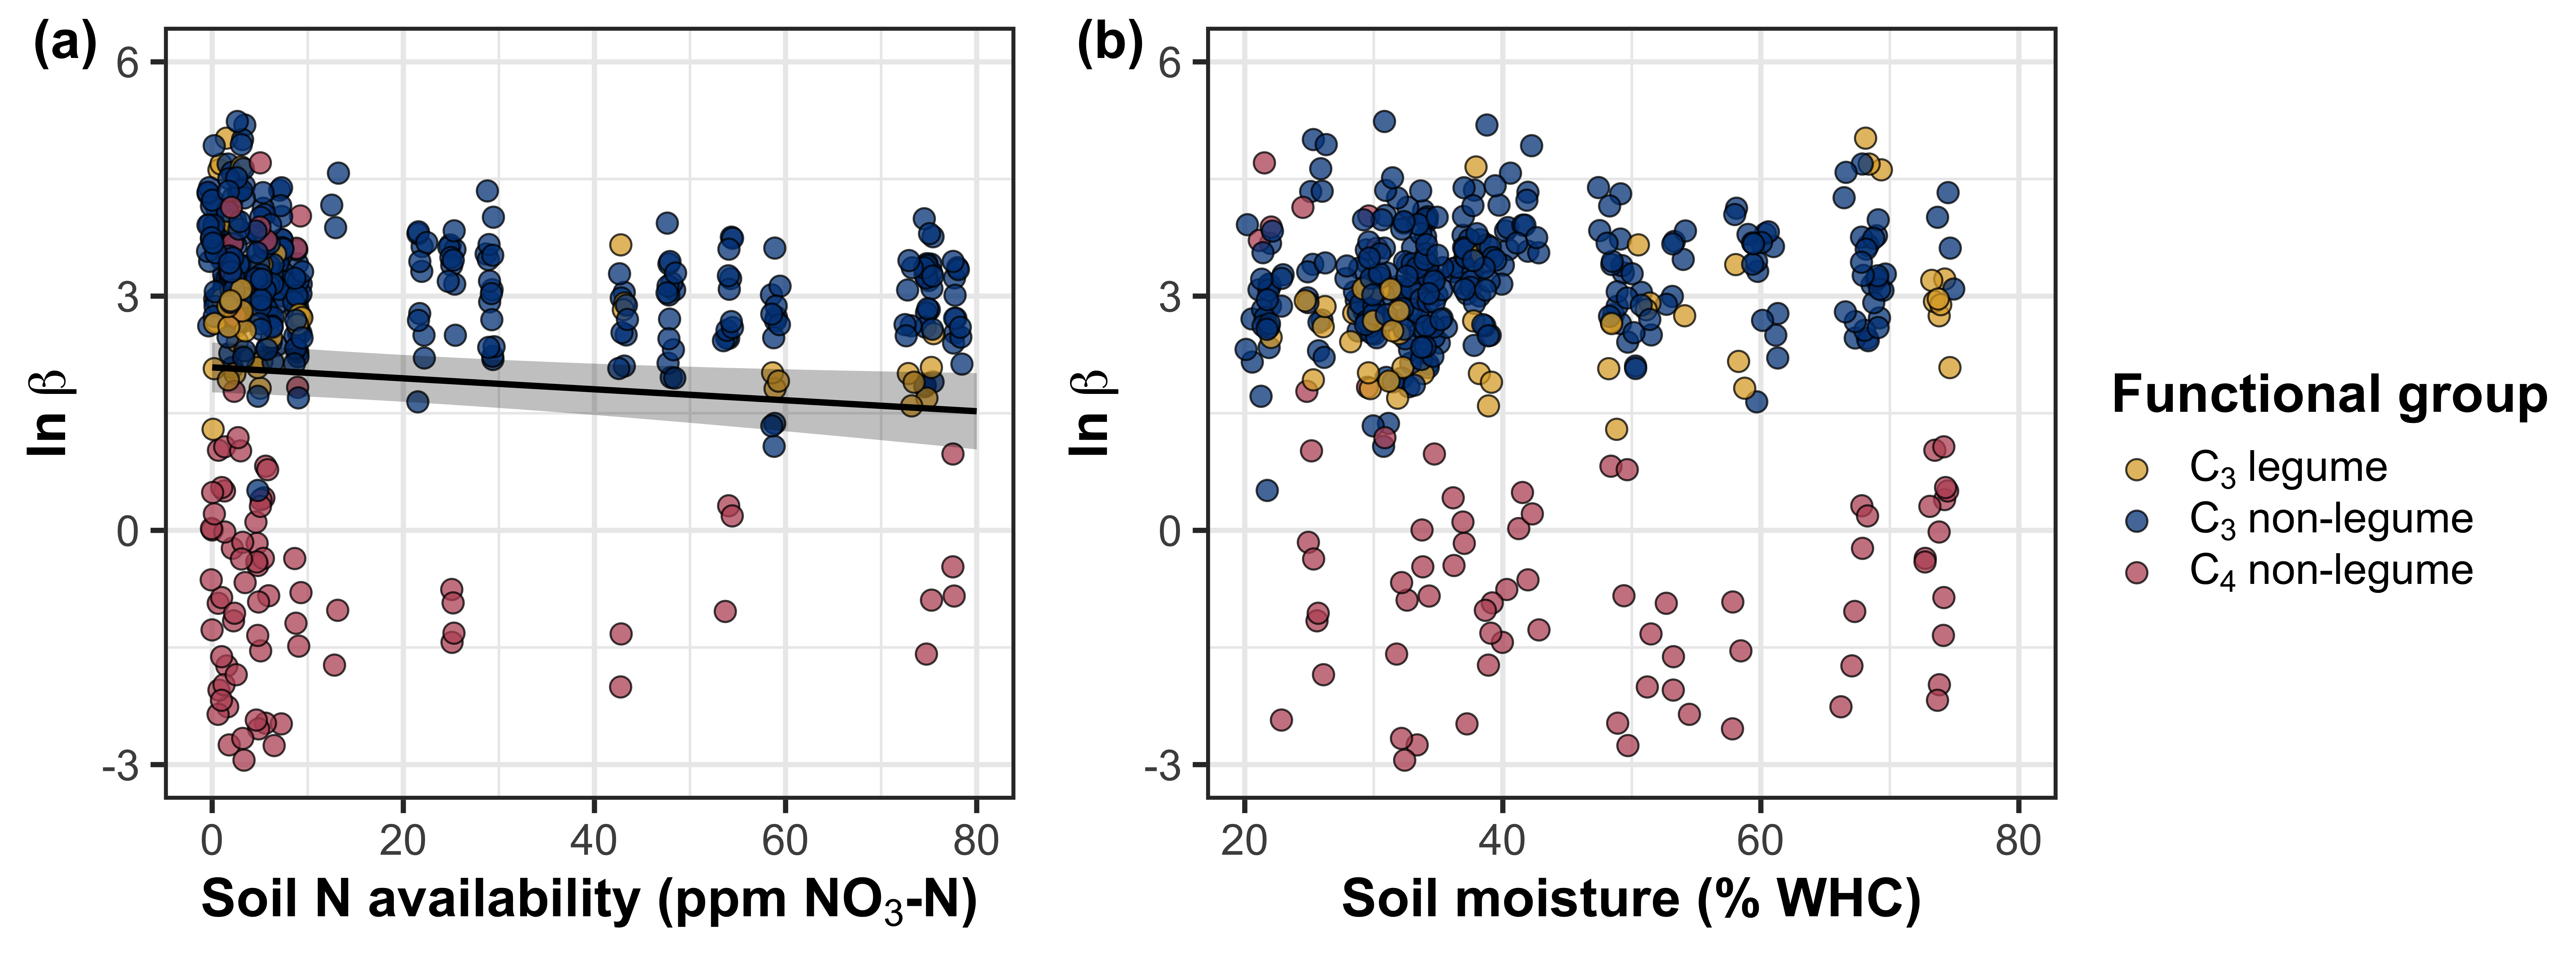
\includegraphics[scale = 0.075]{ch4_TXeco/figs/TXeco_fig2_beta.png}
    \caption[Effects of soil nitrogen availability and soil moisture on the unit cost ratio $\beta$]{Effects of soil nitrogen availability (a) and soil moisture (b) on the unit cost ratio $\beta$. In (b), soil moisture is represented as a percent of site water holding capacity. Yellow shading and trendlines indicate C$_3$ legumes, blue shading and trendlines indicate C$_3$ non-legumes, and red shading and trendlines indicate C$_4$ non-legumes. Points are jittered for visibility. Variably colored trendlines are only included if there is an interaction between the x-axis and plant functional group, where solid trendlines indicate slopes that are different from zero (\textit{p} < 0.05) and dashed trendlines indicate slopes that are not different from zero (\textit{p} < 0.05). Error ribbons represent the upper and lower 95\% confidence intervals of each fitted trendline.}
    \label{fig:figure4.2}
\end{figure}
\end{landscape}
\clearpage

\subsection{\textit{Leaf C\textsubscript{i}:C\textsubscript{a} ($\chi$)}}
Model selection indicated that 4-day daily VPD was the timescale that conferred the best model fit for $\chi$ (AICc = -883.97; Table S1; Fig. S2).

Variance in $\chi$ was driven by a series of two-way interactions between functional group and VPD (\textit{p} = 0.006; Table 3), soil moisture (\textit{p} = 0.033, Table \ref{fig:figure3.3}), and soil nitrogen availability (\textit{p} = 0.022; Table 3). The interaction between 4-day VPD and functional group revealed that the general negative effect of increasing VPD (\textit{p} < 0.001; Table 3) was driven by a negative effect of increasing VPD on $\chi$ in C$_3$ nonlegumes (Tukey: \textit{p} < 0.001) and marginal negative effect in C$_3$ legumes (Tukey: \textit{p} = 0.074) paired with a positive trending, but insignificant effect of increasing VPD in C$_4$ nonlegumes (Tukey: \textit{p} = 0.130; Fig. 3a). The interaction between 2-day soil moisture and functional group indicated that the general negative effect of increasing soil moisture on $\chi$ was driven by a positive effect of increasing soil moisture on $\chi$ in C$_4$ nonlegumes (Tukey: \textit{p} = 0.009) despite a positive trending but insignificant effect of increasing soil moisture on $\chi$ in C$_3$ legumes (Tukey: \textit{p} = 0.116) and a null effect of soil moisture on $\chi$ in C$_3$ nonlegumes (Tukey: \textit{p} = 0.693; Fig. 3c). The interaction between soil nitrogen availability and plant functional group revealed a weak negative effect of increasing soil nitrogen availability on $\chi$ in C$_3$ legumes (Tukey: \textit{p} = 0.045), with no apparent effect in C$_3$ nonlegumes (Tukey: \textit{p} = 0.706) or C$_4$ nonlegumes (Tukey: \textit{p} = 0.757). Finally, an individual effect of functional group (\textit{p} < 0.001; Table 3) revealed that C$_4$ nonlegumes generally had lower $\chi$ than C$_3$ legumes and C$_3$ nonlegumes (Tukey: \textit{p} < 0.001 in both cases), with no apparent difference between C$_3$ legumes and C$_3$ nonlegumes (Tukey: \textit{p} = 0.831).

\newpage
\begin{table}
    \centering
    \caption{Effects of soil moisture, soil nitrogen availability, and plant functional group on $\chi^*$}
    %\resizebox{\columnwidth}{!}{
        \begin{tabular}{p{6cm}p{0.5cm}p{2cm}p{1.5cm}p{1.5cm}}
            \hline 
            & \multicolumn{1}{r}{df} 
            & \multicolumn{1}{r}{Coefficient} 
            & \multicolumn{1}{r}{$\chi^{2}$} 
            & \multicolumn{1}{r}{\textit{p}} 
            \\ 
            \hline
            
            Intercept
            & \multicolumn{1}{r}{-}
            & \multicolumn{1}{r}{9.33E-01}
            & \multicolumn{1}{r}{-}
            & \multicolumn{1}{r}{-}
            \\

            Vapor pressure deficit (VPD\textsubscript{4})
            & \multicolumn{1}{r}{1}
            & \multicolumn{1}{r}{-1.78E-01}
            & \multicolumn{1}{r}{20.792}
            & \multicolumn{1}{r}{\textbf{<0.001}}
            \\

            Soil moisture (SM\textsubscript{2})
            & \multicolumn{1}{r}{1}
            & \multicolumn{1}{r}{4.53E-02}
            & \multicolumn{1}{r}{1.972}
            & \multicolumn{1}{r}{0.160}
            \\

            Soil N (N)
            & \multicolumn{1}{r}{1}
            & \multicolumn{1}{r}{-1.30E-03}
            & \multicolumn{1}{r}{0.168}
            & \multicolumn{1}{r}{0.682}
            \\

            PFT
            & \multicolumn{1}{r}{2}
            & \multicolumn{1}{r}{-}
            & \multicolumn{1}{r}{172.624}
            & \multicolumn{1}{r}{\textbf{<0.001}}
            \\

            SM\textsubscript{2}*N
            & \multicolumn{1}{r}{1}
            & \multicolumn{1}{r}{7.40E-04}
            & \multicolumn{1}{r}{0.849}
            & \multicolumn{1}{r}{0.357}
            \\

            VPD\textsubscript{4}*PFT
            & \multicolumn{1}{r}{2}
            & \multicolumn{1}{r}{-}
            & \multicolumn{1}{r}{10.241}
            & \multicolumn{1}{r}{\textbf{0.006}}
            \\

            SM\textsubscript{2}*PFT
            & \multicolumn{1}{r}{2}
            & \multicolumn{1}{r}{-}
            & \multicolumn{1}{r}{6.806}
            & \multicolumn{1}{r}{\textbf{0.033}}
            \\

            N*PFT
            & \multicolumn{1}{r}{2}
            & \multicolumn{1}{r}{-}
            & \multicolumn{1}{r}{7.602}
            & \multicolumn{1}{r}{\textbf{0.022}}
            \\

            SM\textsubscript{2}*N*PFT
            & \multicolumn{1}{r}{2}
            & \multicolumn{1}{r}{-}
            & \multicolumn{1}{r}{0.732}
            & \multicolumn{1}{r}{0.694}
            \\
            \hline
        \end{tabular}%}
    \label{tab:table4.3}
\end{table}
\noindent \textsuperscript{$*$}Significance determined using Type II Wald $\chi^{2}$ tests ($\alpha$ = 0.05). \textit{P}-values less than 0.05 are in bold and \textit{p}-values where 0.05 < \textit{p} < 0.1 are italicized. $\chi$ was not transformed prior to model fitting, so model coefficients are reported on the response scale. Model coefficients are only included for continuous fixed effects.
\clearpage

\newpage
\begin{figure}
    \centering
    
\includegraphics[scale = 0.07]{ch4_TXeco/figs/TXeco_fig3_chi.png}
    \caption[Effects of 4-day mean vapor pressure deficit, 2-day soil moisture (per water holding capacity), and soil nitrogen availability on $\chi$. ]{Effects of 4-day mean vapor pressure deficit (a), 2-day soil moisture (per water holding capacity; b), and soil nitrogen availability (c) on $\chi$. Shading and trendlines are as explained in Figure 2. Points are jittered for visibility. Variably colored trendlines are only included if there is an interaction between the x-axis and plant functional group, where solid trendlines indicate slopes that are different from zero (\textit{p} < 0.05) and dashed trendlines indicate slopes that are not different from zero (\textit{p} < 0.05). Error ribbons represent the upper and lower 95\% confidence intervals of each fitted trendline.}
    \label{fig:figure4.3}
\end{figure}
\clearpage

\subsection{\textit{Leaf nitrogen content}}
An interaction between $\chi$ and plant functional group (\textit{p} < 0.001; Table 4) revealed that the general negative effect of increasing $\chi$ on $N_\mathrm{area}$ (\textit{p} < 0.001; Table 4) was driven by a negative effect of increasing $\chi$ on $N_\mathrm{area}$ in C$_3$ nonlegumes (Tukey: \textit{p} < 0.001) and C$_3$ legumes (Tukey: \textit{p} = 0.002) despite a null effect of $\chi$ on $N_\mathrm{area}$ in C$_4$ nonlegumes (Tukey: \textit{p} = 0.795; Fig. 4a). An interaction between soil nitrogen availability and soil moisture (\textit{p} = 0.028; Table 4) indicated that the marginal positive effect of increasing soil nitrogen availability on $N_\mathrm{area}$ (\textit{p} = 0.091; Table 4) decreased with increasing soil moisture, despite no apparent individual effect of soil moisture on $N_\mathrm{area}$ (\textit{p} = 0.692; Table 4). Finally, a plant functional group effect (\textit{p} < 0.001; Table 4) indicated that C$_4$ nonlegumes had lower $N_\mathrm{area}$ values on average compared to C$_3$ legumes (Tukey: \textit{p} < 0.001) and C$_3$ nonlegumes (Tukey: \textit{p} = 0.001), while C$_3$ legumes had lower average $N_\mathrm{area}$ values compared to C$_3$ nonlegumes (Tukey: \textit{p} = 0.012).

A marginal interaction between $\chi$ and plant functional group (\textit{p} = 0.088; Table 4) revealed that, despite no apparent general effect of $\chi$ on $N_\mathrm{mass}$ (\textit{p} = 0.273; Table 4), increasing $\chi$ decreased $N_\mathrm{mass}$ in C$_3$ nonlegumes (Tukey: \textit{p} = 0.021), but this effect was not apparent in C$_4$ nonlegumes (Tukey: \textit{p} = 0.693) or C$_3$ legumes (Tukey: p = 0.477). An interaction between soil nitrogen availability and soil moisture (\textit{p} < 0.001; Table 4) indicated that the general positive effect of increasing soil nitrogen availability on $N_\mathrm{mass}$ (\textit{p} < 0.001; Table 4) generally decreased with increasing soil moisture, despite an apparent general positive effect of increasing soil moisture on $N_\mathrm{mass}$ (\textit{p} < 0.001; Table 4). This interaction indicated that the positive effect of increasing soil nitrogen availability on $N_\mathrm{mass}$ was only apparent when soil moisture was less than 70\% the maximum water holding capacity (Tukey: \textit{p} < 0.05 in all cases) despite a positive effect of increasing soil moisture on $N_\mathrm{mass}$ (\textit{p} < 0.001; Table 4). Finally, a plant functional group effect (\textit{p} < 0.001; Table 4) indicated that C$_4$ nonlegumes had lower $N_\mathrm{mass}$ values on average compared to C$_3$ legumes (Tukey: \textit{p} = 0.002) and C$_3$ nonlegumes (Tukey: \textit{p} = 0.019), while $N_\mathrm{mass}$ did not differ between C$_3$ legumes and C$_3$ nonlegumes (Tukey: p = 0.149).

An interaction between $\chi$ and functional group (\textit{p} = 0.005; Table 4) indicated that the general negative effect of increasing $\chi$ on $M_\mathrm{area}$ (\textit{p} < 0.001; Table 4; Fig. 4c) was driven by a negative effect of increasing $\chi$ on $M_\mathrm{area}$ in C$_3$ legumes and C$_3$ nonlegumes (Tukey: \textit{p} < 0.001 in both cases) despite a nonsignificant effect of increasing $\chi$ on $M_\mathrm{area}$ in C$_4$ nonlegumes (Tukey: \textit{p} = 0.724). An interaction between soil nitrogen and soil moisture (\textit{p} < 0.001; Table 4) indicated that the general negative effect of increasing soil nitrogen availability on $M_\mathrm{area}$ (\textit{p} < 0.001; Table 4) decreased with increasing soil moisture, despite an apparent general negative effect of increasing soil moisture on $M_\mathrm{area}$ (\textit{p} = 0.002; Table 4). Specifically, the negative effect of increasing soil nitrogen availability on $M_\mathrm{area}$ was only apparent when soil moisture was less than 65\% the maximum water holding capacity (Tukey: \textit{p} < 0.05 in all cases). An additional interaction between soil nitrogen availability and functional group (\textit{p} = 0.034; Table 4) indicated that the general negative effect of increasing soil nitrogen availability on $M_\mathrm{area}$ was driven by decreases in C$_3$ nonlegumes (Tukey: \textit{p} < 0.001) and C$_4$ nonlegumes (Tukey: \textit{p} = 0.003), with no apparent effect of soil nitrogen availability on $M_\mathrm{area}$ in C$_3$ legumes (Tukey: \textit{p} = 0.997).

\newpage
\begin{landscape}
    \begin{table}
    \centering
    \caption{Effects of soil nitrogen fertilization, inoculation, and CO$_2$ treatments on $N_\mathrm{area}$, $N_\mathrm{mass}$, and $M_\mathrm{area}$}
    \resizebox{\columnwidth}{!}{
        \begin{tabular}{p{3.75cm}p{0.5cm}p{1.75cm}p{1.5cm}p{1.5cm}p{1.75cm}p{1.5cm}p{1.5cm}p{1.75cm}p{1.5cm}p{1.5cm}}
            && 
            \multicolumn{3}{l}{$N_\mathrm{area}$} 
            & \multicolumn{3}{l}{$N_\mathrm{mass}$} 
            & \multicolumn{3}{l}{$M_\mathrm{area}$} 
            \\
            \hline 
            & 
            \multicolumn{1}{r}{df} 
            & \multicolumn{1}{r}{Coefficient}   & \multicolumn{1}{r}{$\chi^{2}$}    & \multicolumn{1}{r}{\textit{p}} 
            & \multicolumn{1}{r}{Coefficient}   & \multicolumn{1}{r}{$\chi^{2}$}    & \multicolumn{1}{r}{\textit{p}} 
            & \multicolumn{1}{r}{Coefficient}   & \multicolumn{1}{r}{$\chi^{2}$}    & \multicolumn{1}{r}{\textit{p}} 
            \\ 
            \hline

            (Intercept) & \multicolumn{1}{r}{-} 
            &  \multicolumn{1}{r}{2.78E+00}     & \multicolumn{1}{r}{-}             & \multicolumn{1}{r}{-}
            &  \multicolumn{1}{r}{4.42E-01}     & \multicolumn{1}{r}{-}             & \multicolumn{1}{r}{-}
            &  \multicolumn{1}{r}{6.97E+00}     & \multicolumn{1}{r}{-}             & \multicolumn{1}{r}{-} 
            \\

            $\chi$ & \multicolumn{1}{r}{1}
            & \multicolumn{1}{r}{-2.53E+00}     & \multicolumn{1}{r}{15.771}        & \multicolumn{1}{r}{\textbf{<0.001}}
            & \multicolumn{1}{r}{4.56E-01}      & \multicolumn{1}{r}{1.201}         & \multicolumn{1}{r}{0.273}
            & \multicolumn{1}{r}{-3.10E+00}     & \multicolumn{1}{r}{20.620}        & \multicolumn{1}{r}{\textbf{<0.001}} 
            \\


            Soil N (N) & \multicolumn{1}{r}{1}
            & \multicolumn{1}{r}{1.08E-02}      & \multicolumn{1}{r}{2.855}         & \multicolumn{1}{r}{\textit{0.091}}
            & \multicolumn{1}{r}{1.37E-02}      & \multicolumn{1}{r}{54.531}        & \multicolumn{1}{r}{\textbf{<0.001}}
            & \multicolumn{1}{r}{-2.87E-03}     & \multicolumn{1}{r}{29.759}        & \multicolumn{1}{r}{\textbf{<0.001}} 
            \\

            Soil moisture (SM\textsubscript{2}) & \multicolumn{1}{r}{1}
            & \multicolumn{1}{r}{3.61E-01}      & \multicolumn{1}{r}{0.157}         & \multicolumn{1}{r}{0.692}
            & \multicolumn{1}{r}{5.04E-01}      & \multicolumn{1}{r}{16.255}        & \multicolumn{1}{r}{\textbf{<0.001}}
            & \multicolumn{1}{r}{-1.26E-01}     & \multicolumn{1}{r}{9.282}         & \multicolumn{1}{r}{\textbf{ 0.002}} 
            \\

            PFT & \multicolumn{1}{r}{1}
            & \multicolumn{1}{r}{-}             & \multicolumn{1}{r}{60.641}        & \multicolumn{1}{r}{\textbf{<0.001}}
            & \multicolumn{1}{r}{-}             & \multicolumn{1}{r}{21.539}        & \multicolumn{1}{r}{\textbf{<0.001}}
            & \multicolumn{1}{r}{-}             & \multicolumn{1}{r}{11.520}        & \multicolumn{1}{r}{\textbf{0.003}} 
            \\

            SM\textsubscript{2}*N & \multicolumn{1}{r}{1}
            & \multicolumn{1}{r}{-1.09E-02}     & \multicolumn{1}{r}{4.779}         & \multicolumn{1}{r}{\textbf{ 0.029}}
            & \multicolumn{1}{r}{-1.76E-02}     & \multicolumn{1}{r}{41.784}        & \multicolumn{1}{r}{\textbf{<0.001}}
            & \multicolumn{1}{r}{6.35E-03}      & \multicolumn{1}{r}{14.111}        & \multicolumn{1}{r}{\textbf{<0.001}} 
            \\

            $\chi$*PFT & \multicolumn{1}{r}{1}
            & \multicolumn{1}{r}{-}             & \multicolumn{1}{r}{15.188}        & \multicolumn{1}{r}{\textbf{<0.001}}
            & \multicolumn{1}{r}{-}             & \multicolumn{1}{r}{4.864}         & \multicolumn{1}{r}{\textit{ 0.088}}
            & \multicolumn{1}{r}{-}             & \multicolumn{1}{r}{17.032}        & \multicolumn{1}{r}{\textbf{ 0.025}} 
            \\

            N*PFT & \multicolumn{1}{r}{1}
            & \multicolumn{1}{r}{-}             & \multicolumn{1}{r}{2.289}         & \multicolumn{1}{r}{0.318}
            & \multicolumn{1}{r}{-}             & \multicolumn{1}{r}{0.914}         & \multicolumn{1}{r}{0.633}
            & \multicolumn{1}{r}{-}             & \multicolumn{1}{r}{6.760}         & \multicolumn{1}{r}{\textbf{0.034}}
            \\

            SM\textsubscript{2}*PFT & \multicolumn{1}{r}{1}
            & \multicolumn{1}{r}{-}             & \multicolumn{1}{r}{0.978}         & \multicolumn{1}{r}{0.613}
            & \multicolumn{1}{r}{-}             & \multicolumn{1}{r}{0.128}         & \multicolumn{1}{r}{0.938}
            & \multicolumn{1}{r}{-}             & \multicolumn{1}{r}{2.121}         & \multicolumn{1}{r}{0.346} 
            \\

            SM\textsubscript{2}*N*PFT & \multicolumn{1}{r}{1}
            & \multicolumn{1}{r}{-}             & \multicolumn{1}{r}{1.289}         & \multicolumn{1}{r}{0.525}
            & \multicolumn{1}{r}{-}             & \multicolumn{1}{r}{2.180}         & \multicolumn{1}{r}{0.336}
            & \multicolumn{1}{r}{-}             & \multicolumn{1}{r}{0.629}         & \multicolumn{1}{r}{0.730}
            \\
            \hline

    \end{tabular}}
    \label{tab:table4.4}
    \end{table}
    \noindent \textsuperscript{$*$}Significance determined using Type II Wald $\chi^{2}$ tests ($\alpha$ = 0.05). \textit{P}-values less than 0.05 are in bold and \textit{p}-values where 0.05 < \textit{p} < 0.1 are italicized. Coefficients are reported on the natural-log scale and are only included for continuous fixed effects.
\end{landscape}
\clearpage

\newpage
    \begin{figure}
        \centering
        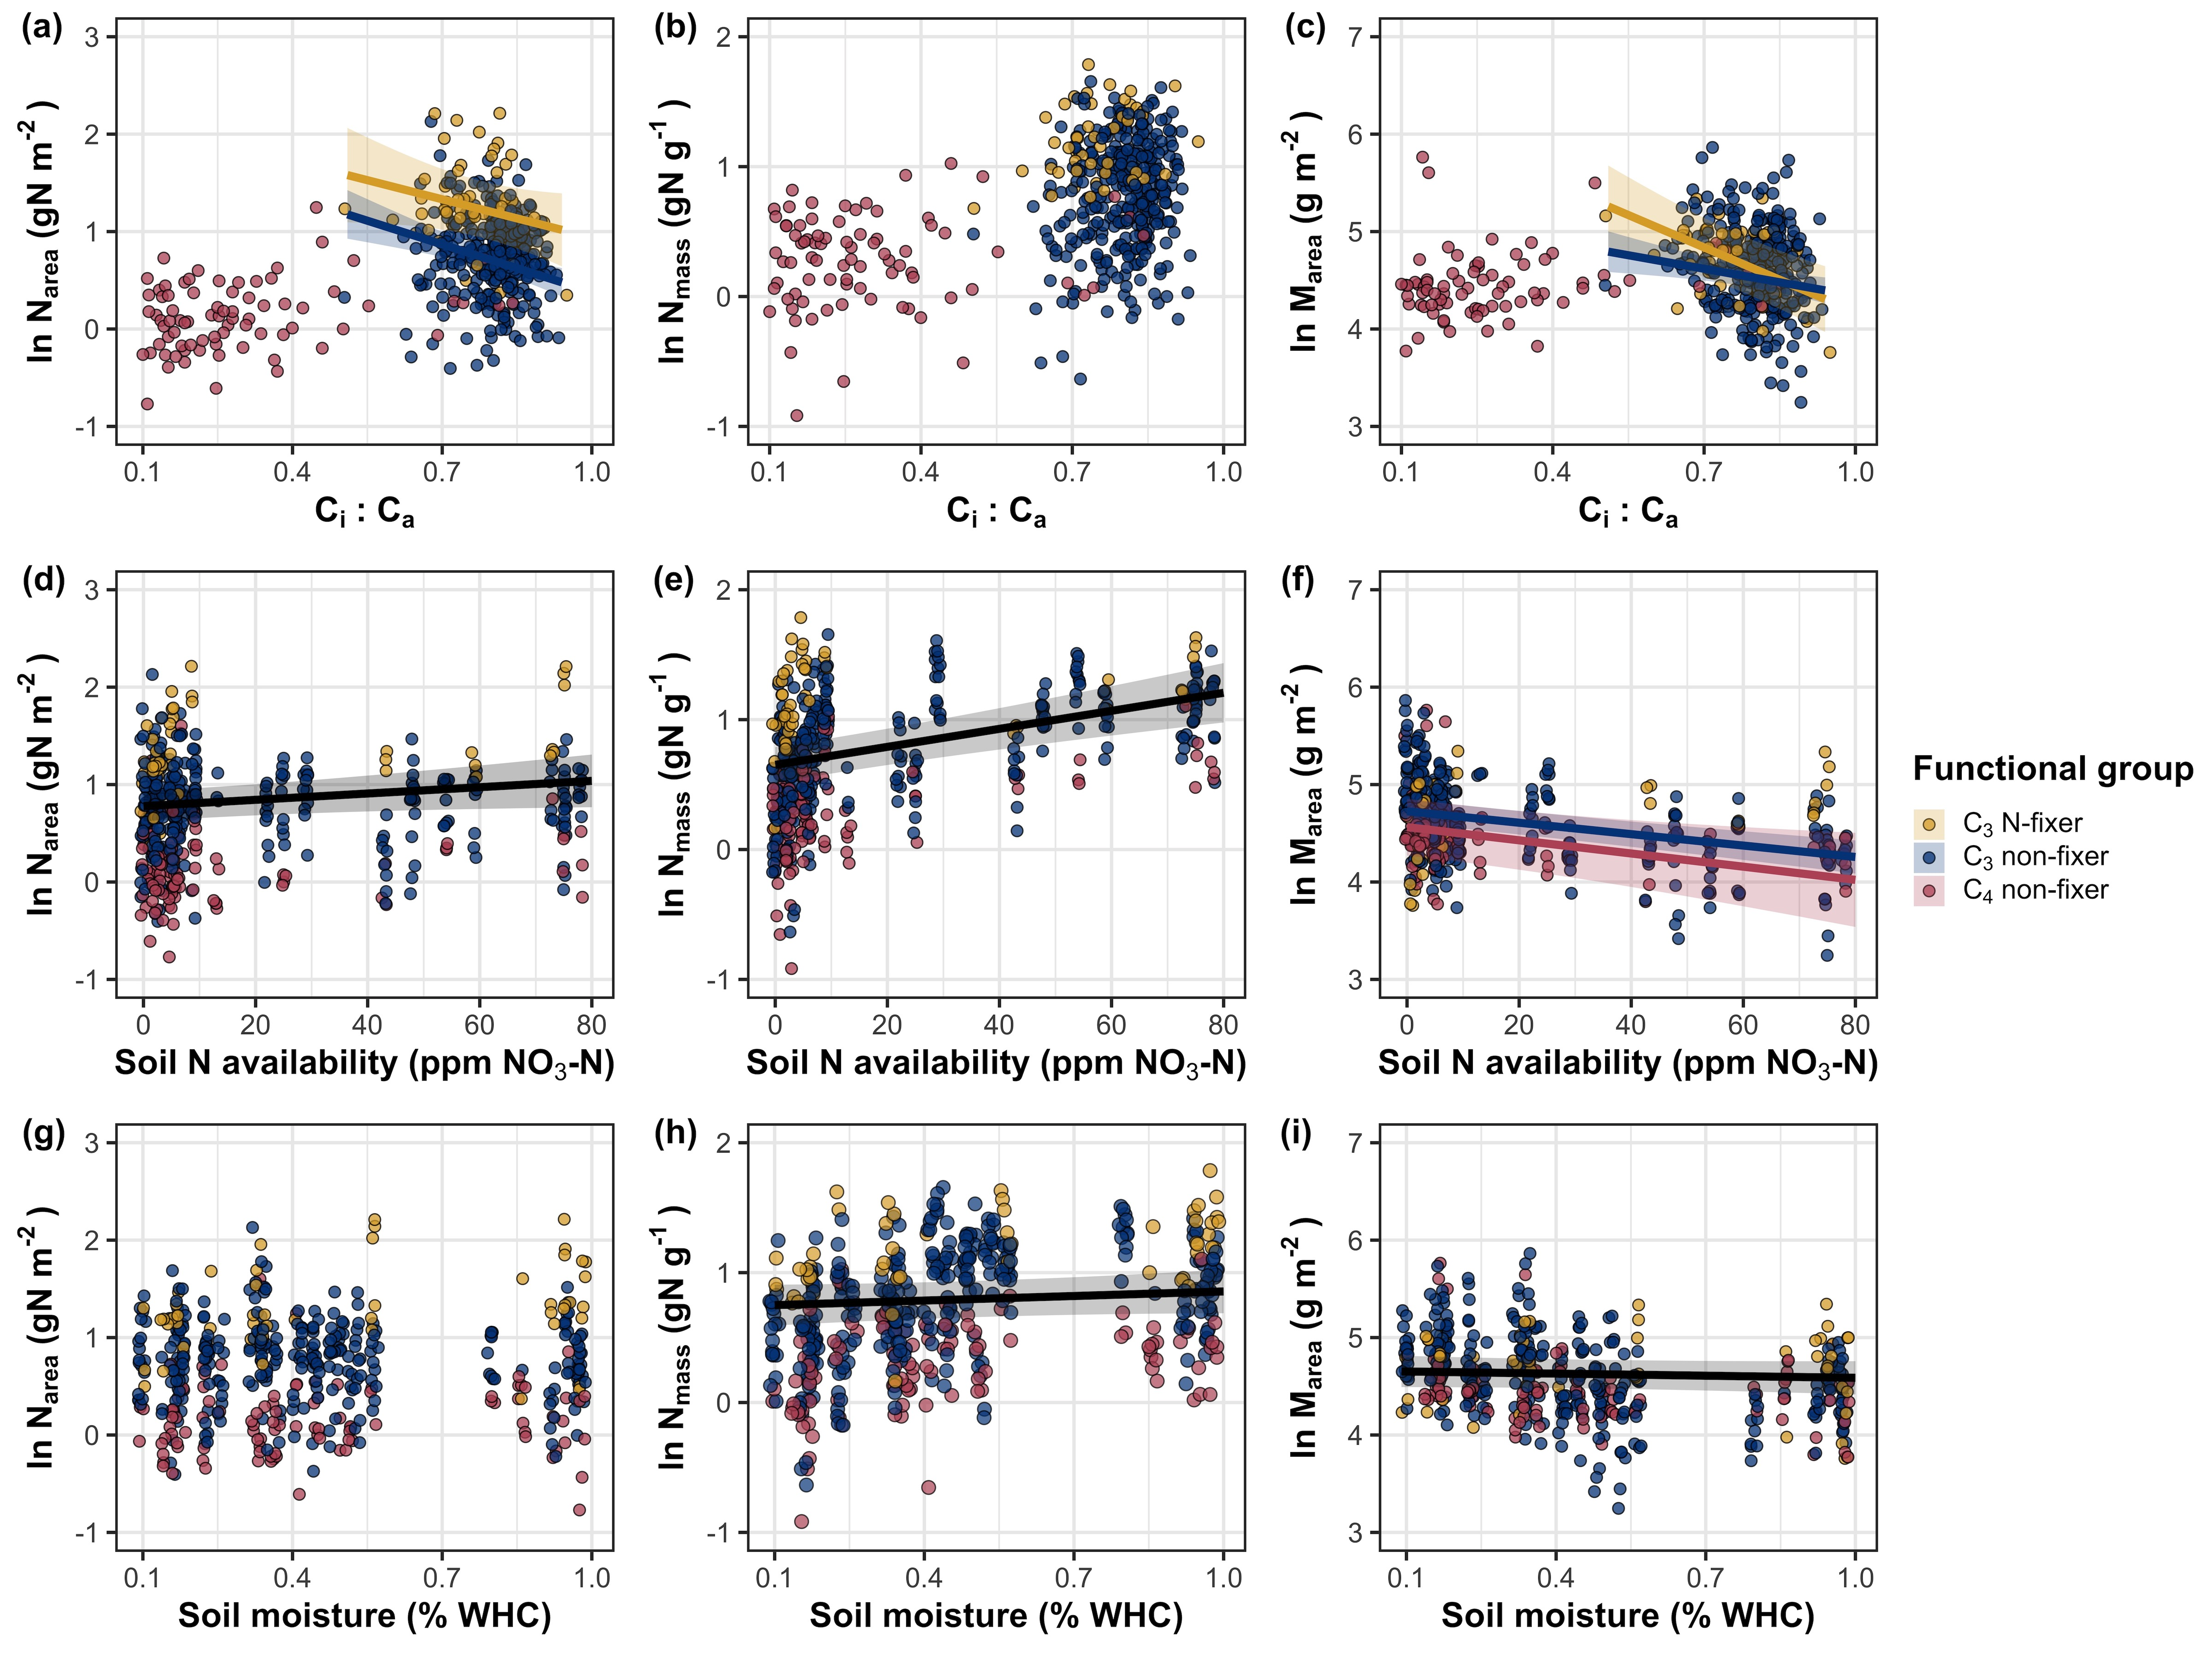
\includegraphics[scale = 0.042]{ch4_TXeco/figs/TXeco_fig4_narea.png}
        \caption[Effects of $\chi$, soil nitrogen availability, and soil moisture on leaf nitrogen content per unit leaf area, leaf nitrogen content per unit leaf biomass, and leaf mass per area.]{Effects of $\chi$ (a-c), soil nitrogen availability (d-f), and soil moisture (g-i) on leaf nitrogen content per unit leaf area (a, d, g), leaf nitrogen content per unit leaf biomass (b, e, h), and leaf mass per area (c, f, i). A solid black trendline indicates the bivariate relationship between the fixed effect the x-axis and response variable on the y-axis and is only included when there is no interaction between the x-axis and plant functional group.}
        \label{fig:figure4.4}
    \end{figure}
\clearpage

\subsection{\textit{Structural equation model}}
The piecewise structural equation model explained 90\%, 54\%, 80\%, 92\%, and 41\% of variance in $N_\mathrm{area}$, $N_\mathrm{mass}$, $M_\mathrm{area}$, $\chi$, and $\beta$, respectively (Table 5; Fig. 5). Variance in $N_\mathrm{area}$ was driven by a negative effect of increasing $\chi$ (\textit{p} < 0.001; Table 5) paired with positive effects of increasing $N_\mathrm{mass}$ and $M_\mathrm{area}$ (\textit{p} < 0.001 in both cases; Table 5; Fig. 5). Model results indicated that the negative effect of $\chi$ on $N_\mathrm{area}$ was driven by a strong reduction in $M_\mathrm{area}$ with increasing $\chi$ (\textit{p} < 0.001; Table 5) paired with no change in $\chi$ due to $N_\mathrm{mass}$ (\textit{p} = 0.150; Table 5). However, there was a strong negative effect of increasing $M_\mathrm{area}$ on $N_\mathrm{mass}$ (\textit{p} < 0.001; Table 5; Fig. 5). $\chi$ generally increased with increasing $\beta$  (\textit{p} < 0.001; Table 5) and decreased with increasing VPD (\textit{p} < 0.001; Table 5; Fig. 5). Variance in $\beta$  was driven by a negative effect of increasing soil nitrogen availability (\textit{p} < 0.001; Table 5) and was generally higher in C$_3$ species (\textit{p} < 0.001; Table 5; Fig. 5). However, $\beta$ did not change with soil moisture (\textit{p} = 0.332; Table 5) or with ability to acquire nitrogen via symbiotic nitrogen fixation (\textit{p} = 0.546; Table 5). Finally, soil nitrogen availability was positively associated with increasing soil moisture (\textit{p} < 0.001; Table 5; Fig. 5), while VPD was negatively associated with increasing soil moisture (\textit{p} < 0.001; Table 5; Fig. 5).

\newpage
\begin{table}
    \centering
    \caption{Structural equation model results investigating direct effects of climatic and soil resource availability on $N_\mathrm{area}$, $N_\mathrm{mass}$, $M_\mathrm{area}$, $\chi$, and $\beta$}
    %\resizebox{\columnwidth}{!}{
        \begin{tabular}{p{0.5cm}p{3cm}p{1.5cm}p{1.5cm}}
            \hline
            & Predictor & \multicolumn{1}{r}{Coefficient} & \multicolumn{1}{r}{\textit{p}} \\
            \hline

            \multicolumn{2}{l}{$N_\mathrm{area}$ ($R^2{}_c$) = 0.90} && \\
            & \multicolumn{1}{l}{$\chi$} & \multicolumn{1}{r}{-0.140} & \multicolumn{1}{r}{\textbf{<0.001}} \\
            & \multicolumn{1}{l}{$M_\mathrm{area}$} & \multicolumn{1}{r}{0.807} & \multicolumn{1}{r}{\textbf{<0.001}} \\
            & \multicolumn{1}{l}{$N_\mathrm{mass}$} & \multicolumn{1}{r}{0.795} & \multicolumn{1}{r}{\textbf{<0.001}} \\
            \hline

            \multicolumn{2}{l}{$N_\mathrm{mass}$ ($R^2{}_c$) = 0.54} && \\
            & \multicolumn{1}{l}{$\chi$} & \multicolumn{1}{r}{0.097} & \multicolumn{1}{r}{\textbf{<0.001}} \\
            \hline

            \multicolumn{2}{l}{$M_\mathrm{area}$ ($R^2{}_c$) = 0.80} && \\
            & \multicolumn{1}{l}{$\chi$} & \multicolumn{1}{r}{-0.372} & \multicolumn{1}{r}{0.150} \\
            & \multicolumn{1}{l}{$M_\mathrm{area}$} & \multicolumn{1}{r}{-0.303} & \multicolumn{1}{r}{\textbf{<0.001}} \\
            \hline

            \multicolumn{2}{l}{$\chi$ ($R^2{}_c$) = 0.92} && \\
            & \multicolumn{1}{l}{$\beta$} & \multicolumn{1}{r}{0.261} & \multicolumn{1}{r}{\textbf{<0.001}} \\
            & \multicolumn{1}{l}{VPD\textsubscript{4}} & \multicolumn{1}{r}{-0.122} & \multicolumn{1}{r}{\textbf{<0.001}} \\
            \hline

            \multicolumn{2}{l}{$\beta$ ($R^2{}_c$) = 0.41} && \\
            & \multicolumn{1}{l}{Soil N} & \multicolumn{1}{r}{-0.201} & \multicolumn{1}{r}{\textbf{<0.001}} \\
            & \multicolumn{1}{l}{SM\textsubscript{2}} & \multicolumn{1}{r}{-0.048} & \multicolumn{1}{r}{0.332} \\
            & \multicolumn{1}{l}{Photo. pathway} & \multicolumn{1}{r}{0.490} & \multicolumn{1}{r}{\textbf{<0.001}} \\
            & \multicolumn{1}{l}{N-fixing ability} & \multicolumn{1}{r}{-0.053} & \multicolumn{1}{r}{0.546} \\
            \hline

            \multicolumn{2}{l}{Soil N ($R^2{}_c$) = 0.39} && \\
            & \multicolumn{1}{l}{SM\textsubscript{2}} & \multicolumn{1}{r}{0.410} & \multicolumn{1}{r}{\textbf{<0.001}} \\
            \hline

        \end{tabular}%}
        \label{tab:table4.5}
    \end{table}
\begin{singlespace}
    \noindent \textsuperscript{$*$}Reported coefficients are standardized across the structural equation model. \textit{P}-values less than 0.05 are noted in bold. Positive coefficients for photosynthetic pathway indicate generally larger values in C\textsubscript{3} species, while positive coefficients for N-fixing ability indicate generally larger values in N-fixing species. Key: $N_\mathrm{area}$=leaf nitrogen content per unit leaf area, $M_\mathrm{area}$=leaf mass per unit leaf dry biomass, $N_\mathrm{mass}$=leaf nitrogen content per unit leaf dry biomass, $\beta$=cost of acquiring nitrogen relative to water, $\chi$=isotope-derived estimate of the leaf Ci:Ca ratio, VPD\textsubscript{4}= 4-day mean vapor pressure deficit, SM\textsubscript{2}=2-day mean soil moisture, R\textsuperscript{2}\textsubscript{c} = conditional R\textsuperscript{2} value
\end{singlespace}
\clearpage

\newpage
\begin{landscape}
    \begin{figure}
        \centering
        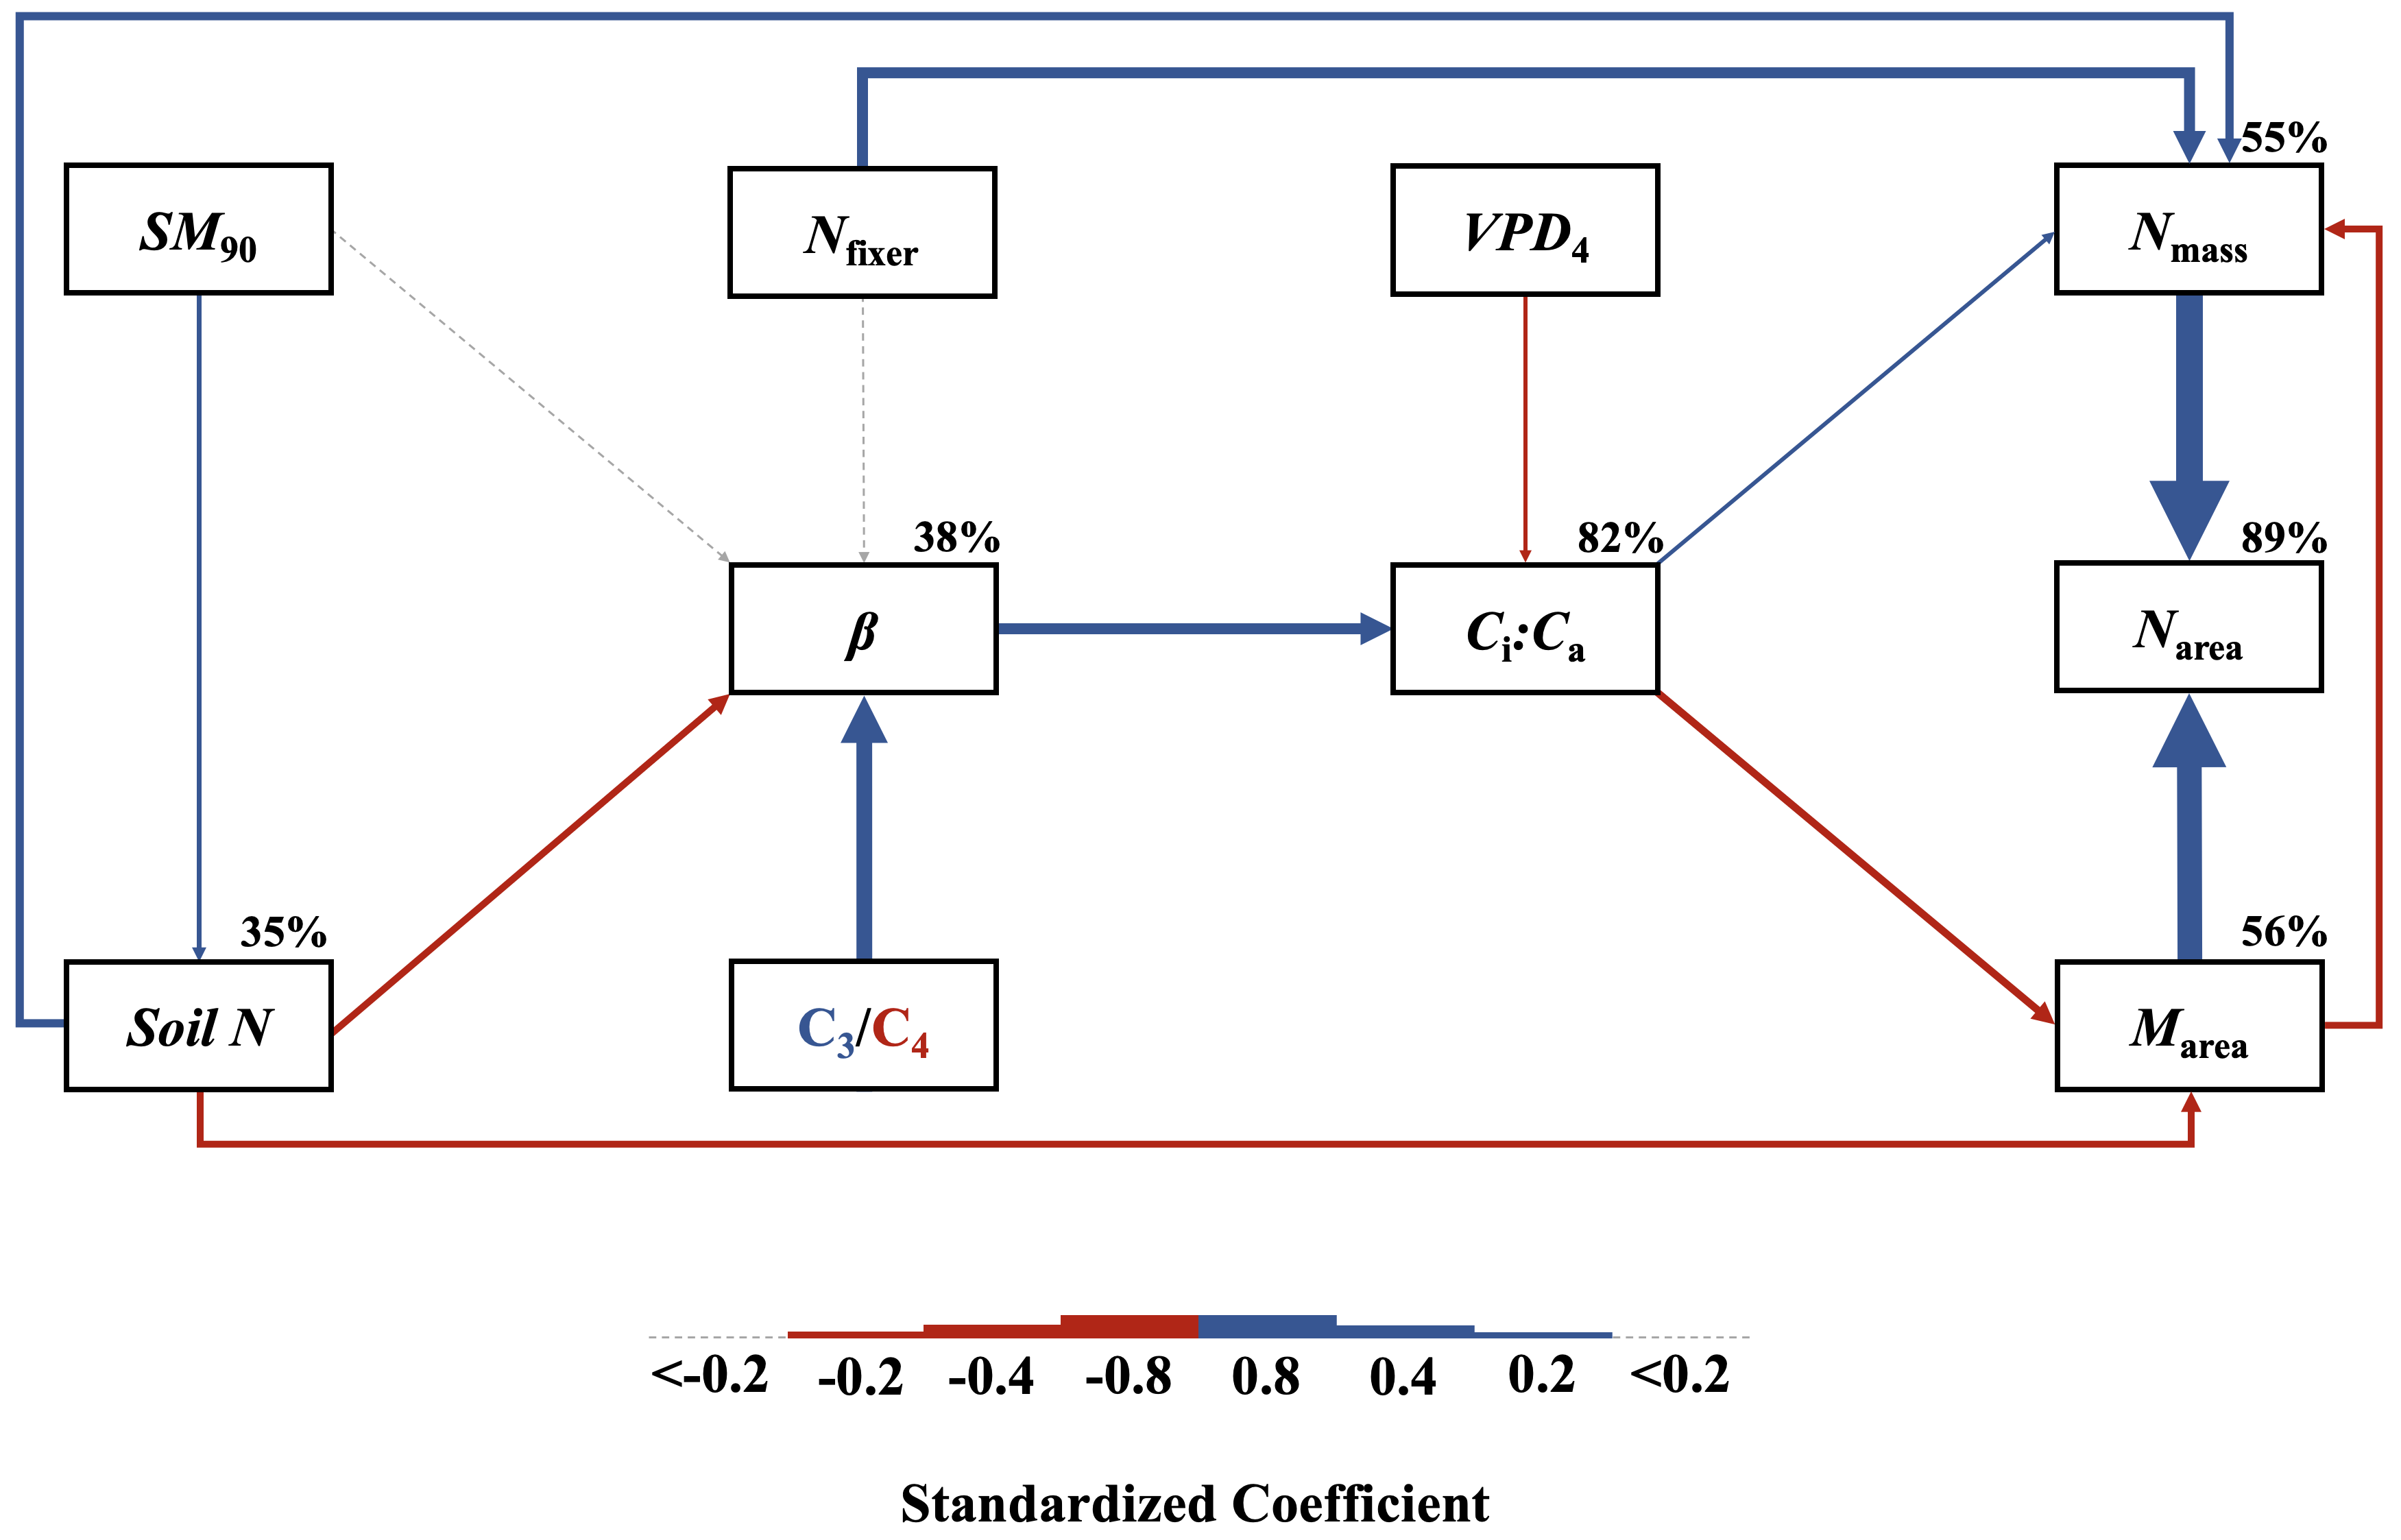
\includegraphics[scale = 0.3]{ch4_TXeco/figs/TXeco_fig5_SEM.png}
        \caption[Structural equation model results exploring direct and indirect drivers of $N_\mathrm{area}$]{Structural equation model results exploring direct and indirect drivers of $N_\mathrm{area}$. Boxes indicate measured edaphic factors, climatic factors, and leaf traits. Percentages above boxes indicate conditional $R^{2}$ values of each respective leaf trait. Solid arrows indicate bivariate relationships where \textit{p} < 0.05, while dashed arrows indicate bivariate relationships where \textit{p} > 0.05. Positive model coefficients are indicated through blue arrows, while negative model coefficients are indicated through red arrows. Arrow thickness scales with the standardized model coefficient of each bivariate relationship. A positive coefficient for photosynthetic pathway indicates generally larger values in C$_3$ species, while a positive coefficient for $N_\mathrm{fixer}$ indicates generally larger values in N-fixing species. Standardized model coefficients and associated \textit{p}-values are reported in Table 5.}
        \label{fig:figure4.5}
    \end{figure}
\end{landscape}
\clearpage


\section{Discussion}
In this study, we quantified direct and indirect effects of soil resource availability, climate, $\chi$, and $\beta$ on $N_\mathrm{area}$ and components of $N_\mathrm{area}$ ($N_\mathrm{mass}$ and $M_\mathrm{area}$) in 520 individuals spanning across a soil resource availability and climate gradient in Texas, USA. We found consistent support for patterns expected from photosynthetic least-cost theory, a result driven by a strong direct negative relationship between the relative costs to acquire nitrogen versus water ($\beta$) on $N_\mathrm{area}$ as mediated through changes in the leaf C\textsubscript{i}:C\textsubscript{a} ratio ($\chi$). In further support of patterns expected from theory, increasing soil nitrogen availability had a strong negative effect on $\beta$, resulting in an indirect stimulation in $N_\mathrm{area}$. Increasing VPD also indirectly increased $N_\mathrm{area}$ through a direct negative effect of increasing VPD on $\chi$. Interestingly, we found a strong positive association between soil moisture and soil nitrogen availability resulted in an indirect positive effect of increasing soil moisture on $N_\mathrm{area}$ despite an apparent null direct effect of soil moisture on $N_\mathrm{area}$. Overall, results provide strong and consistent support for patterns expected from photosynthetic least-cost theory, showing that both soil resource availability and climate drive variance in $N_\mathrm{area}$ through changes in $\chi$.

\subsection{\textit{Negative effects of $\chi$ on $N_\mathrm{area}$ are driven by reductions in $M_\mathrm{area}$, not $N_\mathrm{mass}$}}
A strong negative effect of increasing $\chi$ on $N_\mathrm{area}$ was detected in both the linear mixed effect and piecewise structural equation models. The negative response of $N_\mathrm{area}$ to increasing $\chi$ is consistent with previous environmental gradient \shortcite{Dong2017,Querejeta2022} and manipulation experiments (Perkowski et al. n.d.), showing strong support for the nitrogen-water use tradeoffs expected from photosynthetic least cost theory \shortcite{Wright2003,Prentice2014}. Negative effects of increasing $\chi$ on $N_\mathrm{area}$ were driven by a strong negative effect of increasing $\chi$ on $M_\mathrm{area}$, with no apparent effect of $\chi$ on $N_\mathrm{mass}$, suggesting that changes in $N_\mathrm{area}$ were driven by changes in leaf structure and not leaf chemistry. Interestingly, increasing $M_\mathrm{area}$ was negatively associated with $N_\mathrm{mass}$, indicating that an increase in $N_\mathrm{mass}$ was associated with larger, thinner leaves (i.e. lower $M_\mathrm{area}$). These results are consistent with patterns reported from previous studies indicating that variance in $N_\mathrm{area}$ is driven by changes in $M_\mathrm{area}$ across environmental gradients, and that part of this response is due to negative covariance between $M_\mathrm{area}$ and $N_\mathrm{mass}$ associated with tradeoffs between leaf longevity and leaf productivity \shortcite{Wright2004,Dong2017,Dong2022a,Wang2023,Querejeta2022}.

The negative relationship between $\chi$ and $M_\mathrm{area}$ could be also response that allows leaves to maximize productivity in shorter-lived leaves. Tradeoffs between leaf longevity and leaf productivity are commonly observed and are included in a continuum of coordinated leaf traits that position individuals along a fast- or slow-growing leaf economics spectrum \shortcite{Wright2004,Onoda2004,Onoda2017,Reich2014,Wang2023}. Negative relationships between $\chi$ and $M_\mathrm{area}$ indicate that increased stomatal conductance and reduced water use efficiency were associated with thinner, larger leaves (i.e., lower $M_\mathrm{area}$). These patterns, combined with the negative relationship between $M_\mathrm{area}$ and $N_\mathrm{mass}$ mentioned above, likely allowed individuals to maximize light interception and productivity by exploiting high light environments, though this may come at the expense of increased water loss and decreased water-use efficiency. This strategy may be especially advantageous for fast-growing species in open canopy systems. In this study, C$_3$ legumes and C$_3$ nonlegumes dominated the dataset (78\% of total sampling effort), of which 22\% (17\% of total sampling effort) were classified as annual species with short growing seasons. We observed no effect of $\chi$ on $N_\mathrm{area}$ or $M_\mathrm{area}$ in C$_4$ nonlegumes, which made up 22\% of the sampling effort and were generally classified as warm season graminoid species with slower growth rates and longer growing seasons. These patterns indicate that stronger tradeoffs between nitrogen and water use may be more apparent in fast-growing species with high demand for building and maintaining productive leaf tissues.

\subsection{\textit{Soil nitrogen availability increases $N_\mathrm{area}$ through changes in the cost to acquire nitrogen}}
The null effect of soil nitrogen availability on $N_\mathrm{area}$ was driven by positive and negative respective effects of increasing soil nitrogen availability on $N_\mathrm{mass}$ and $M_\mathrm{area}$ that were equal in magnitude. The null response of $N_\mathrm{area}$ to soil nitrogen availability occurred alongside a negative effect of increasing soil nitrogen availability on $\beta$, which, paired with the negative relationship between $\chi$ and $N_\mathrm{area}$, suggests a general positive effect of increasing soil nitrogen availability on $N_\mathrm{area}$, but only when mediated through changes in $\beta$. This result is consistent with our hypotheses and patterns expected from photosynthetic least-cost theory. These results suggest that positive direct effects of increasing soil nitrogen availability on $N_\mathrm{area}$ are not ubiquitous across environmental gradients. Instead, as predicted by our hypotheses and patterns expected from theory, positive responses of $N_\mathrm{area}$ to increasing soil nitrogen availability are a deterministic acclimation response to shifts in climate-related demand to build and maintain photosynthetic enzymes, which allows plants to optimize photosynthetic processes and resource use to a given environment \shortcite{Paillassa2020,Peng2021,Dong2022a,Westerband2023}.

\subsection{\textit{Soil moisture increases $N_\mathrm{area}$ by facilitating increases in soil nitrogen availability}}
Increasing soil moisture generally had no effect on $N_\mathrm{area}$, a response that was associated with a null effect of soil moisture on $\beta$. These results contrast patterns expected from theory, where increasing soil moisture is expected to indirectly decrease $N_\mathrm{area}$ through an increase in $\beta$ due to a reduction in costs associated with water acquisition and use \shortcite{Wright2003,Prentice2014,Lavergne2020}. Interestingly, structural equation model results revealed a strong positive association between soil moisture and soil nitrogen availability, indicating an indirect positive effect of increasing soil moisture on $N_\mathrm{area}$ mediated by the negative effect of increasing soil nitrogen availability on $\beta$. In Texan grasslands, productivity and nutrient uptake are often co-limited by precipitation and nutrient availability \shortcite{Yahdjian2011,Wang2017_NPP_stability}. Thus, increases in soil moisture may have facilitated more favorable and productive environments for soil microbial communities, thereby stimulating the accumulation of plant-available nitrogen substrate through increased ammonification or nitrification rates \shortcite{Reichman1966,Stark1995,Paul2003}. Alternatively, soil moisture may have facilitated greater nitrogen mobility through soil solution. As discussed above, the positive indirect response of $N_\mathrm{area}$ to increasing soil nitrogen availability as mediated through reductions in $\beta$ follow patterns expected from theory.

\subsection{\textit{Indirect effects of climate on $N_\mathrm{area}$ are mediated through changes in leaf C\textsubscript{i}:C\textsubscript{a} and $\beta$}}
In support of our hypothesis and patterns expected from theory, increasing VPD indirectly increased $N_\mathrm{area}$, mediated through the negative effect of increasing VPD on $\chi$. These responses are consistent with previous work noting strong reductions in stomatal conductance with increasing VPD \shortcite{Oren1999,Novick2016,Sulman2016,Grossiord2020}, a response that allows plants to minimize water loss as a result of high atmospheric water demand. Results also support findings from previous experiments across environmental gradients, where increasing VPD generally increases $N_\mathrm{area}$ at lower stomatal conductance across environmental gradients \shortcite{Dong2017,Dong2022a,Paillassa2020,Westerband2023}.

\subsection{\textit{Species identity traits modify effects of the environment on $\beta$, $\chi$, and $N_\mathrm{area}$}}
N-fixing species generally had higher $N_\mathrm{area}$ values on average compared to non-fixing species, a pattern driven by a stronger stimulation in $N_\mathrm{mass}$ in N-fixing species coupled with no change in $M_\mathrm{area}$ between species with different N-fixation ability. We found no evidence to suggest that N-fixing species had different $\beta$ or $\chi$ values compared to non-fixing species across the environmental gradient. These results follow patterns from previous environmental gradient experiments that investigate variance in leaf nitrogen allocation in N-fixing species \shortcite{Adams2016,Dong2017,Dong2020}, and that increases in $N_\mathrm{mass}$ and $N_\mathrm{area}$ in N-fixing species are not necessarily correlated to increases in water use efficiency or reductions in $\chi$ \shortcite{Adams2016}. While our results are consistent with results from previous environmental gradient experiments, they do not necessarily support our hypothesis or patterns expected form theory, which predicts that stimulations in $N_\mathrm{area}$ by N-fixing species should be driven by a reduction in $\beta$ relative to non-fixing species, and that this response should decrease stomatal conductance and $\chi$.

C\textsubscript{4} species generally had lower $\beta$, $\chi$, and $N_\mathrm{area}$ values than C\textsubscript{3} species. Reduced $\beta$ and $\chi$ values in C\textsubscript{4} species follow our hypothesis, a pattern that could be the result of either reduced costs of nitrogen acquisition and use or increased costs of water acquisition and use or both \shortcite{Wright2003,Prentice2014}. Results also indicate that $\beta$ in C\textsubscript{4} nonlegumes was unresponsive to changes in soil nitrogen availability despite an apparent negative effect of increasing soil nitrogen availability on $\beta$ in C\textsubscript{3} legumes and C\textsubscript{3} nonlegumes. Combined with a general null response of $\beta$ to soil moisture regardless of plant functional group, these patterns imply that reduced $\beta$ values in C\textsubscript{4} species may be the result of lower costs of nitrogen acquisition and use relative to C\textsubscript{3} species. While lower $\beta$ values in C\textsubscript{4} species provides a possible explanation for why C\textsubscript{4} species often have lower $\chi$ and greater water use efficiency, theory predicts that this response should cause C\textsubscript{4} species to have greater $N_\mathrm{area}$ values compared to C\textsubscript{3} species, though C\textsubscript{4} species commonly exhibit lower $N_\mathrm{area}$ and higher nitrogen use efficiency than C\textsubscript{3} species \shortcite{Schmitt1981,Sage1987_c3c4,Ghannoum2011}. We speculate that lowered costs of nitrogen acquisition and use in C\textsubscript{4} species could be driven by more efficient Rubisco carboxylation efficiency in C\textsubscript{4} species associated with CO2 concentrating mechanisms that eliminate photorespiration \shortcite{Ghannoum2011}, which could reduce or eliminate the need to sacrifice inefficient nitrogen use for efficient water use to achieve optimal photosynthesis rates.

\subsection{\textit{Next steps for optimality model development}}
Optimality models for both C\textsubscript{3} and C\textsubscript{4} species have been developed using principles from photosynthetic least-cost theory \shortcite{Prentice2014,Wang2017,Smith2019,Stocker2020,Scott2022}. In both C\textsubscript{3} and C\textsubscript{4} model variants, $\beta$ values are held constant using global datasets of leaf $\delta^{13}$C \shortcite{Wang2017,Cornwell2018}. Specifically, the C\textsubscript{3} optimality model initially assumed a constant $\beta$ value of 240 \shortcite{Wang2017}, later corrected to 146 \shortcite{Stocker2020}, while the C\textsubscript{4} optimality model assumes a constant $\beta$ value of 166 \shortcite{Scott2022}. Our results, which build on findings from \shortciteN{Paillassa2020}, demonstrate high variability in calculated $\beta$ values across environmental gradients. Specifically, $\beta$ values in C\textsubscript{3} species ranged from 1.7 to 188.0 (mean: 30.2; median: 23.1; standard deviation: 25.4), while ranged from 0.1 to 110.6 in C\textsubscript{4} species (mean: 7.2; median: 0.7; standard deviation: 18.6). Mean $\beta$ values in both C\textsubscript{3} and C\textsubscript{4} species were consistently lower than values currently implemented in optimality models, though this was likely the result of increased water limitation across our sites relative to global averages. Regardless, the high degree of $\beta$ variability across this environmental gradient, together with findings from \shortciteN{Lavergne2020} and \shortciteN{Paillassa2020}, suggests that the use of constant $\beta$ values may contribute to erroneous errors when conducting optimality model simulations. We therefore build on suggestions from \shortciteN{Wang2017}, recommending future photosynthetic least-cost model developments to consider the use of dynamic $\beta$ values.

\subsection{\textit{Conclusions}}
To summarize, variability in Narea across an environmental gradient in Texan grasslands was driven by indirect effects of climate and soil resource availability mediated. Results from this experiment provide strong and consistent support for patterns expected from photosynthetic least-cost theory, demonstrating that negative relationships between $\chi$ and $N_\mathrm{area}$ unify expected effects of climatic and edaphic characteristics on Narea across environmental gradients. Our results also demonstrate a need to consider the dynamic nature of the relative cost of nitrogen versus water uptake ($\beta$) across environmental gradients in optimality models that leverage principles of photosynthetic least-cost theory.